\documentclass[journal=jctcce,manuscript=article]{achemso}
\setkeys{acs}{articletitle=true}
\SectionNumbersOn

\usepackage{amsmath}
\usepackage{multirow}
\usepackage{xspace}
\usepackage{booktabs}
\usepackage{float}
\usepackage{subfig}
\usepackage{textcomp}
\usepackage{color}
\usepackage{hyperref}
\newcommand{\textapprox}{\raisebox{0.5ex}{\texttildelow}}


\newcommand{\qcaN}{QCArchive}
\newcommand{\qcelN}{QCElemental}
\newcommand{\qcskN}{QCSchema}
\newcommand{\qcngN}{QCEngine}
\newcommand{\qcfN}{QCFractal}
\newcommand{\qcptlN}{QCPortal}


\newcommand{\qca}{{\sc{\qcaN}}\xspace}%
\newcommand{\qcai}{{\sc{\qcaN\xspace Infrastructure}}\xspace}%
\newcommand{\qcsk}{{\sc{\qcskN}}\xspace}%
\newcommand{\qcel}{{\sc{\qcelN}}\xspace}%
\newcommand{\qcng}{{\textsc{\qcngN}}\xspace}%
\newcommand{\qcf}{{\sc{\qcfN}}\xspace}%
\newcommand{\qcptl}{{\sc{\qcptlN}}\xspace}%
\newcommand{\mqcas}{{\sc{mqcas}}\xspace}%

\graphicspath{ {./images/} }

\title{The MolSSI \qca Project: An open-source platform to compute, organize, and share quantum chemistry data}
\author{Daniel G. A. Smith}
\email{dgasmith@vt.edu}
\affiliation{
    Molecular Sciences Software Institute,
    Blacksburg, Virginia 24060, USA}
\author{Doaa Altarawy}
\affiliation{
    Molecular Sciences Software Institute,
    Blacksburg, Virginia 24060, USA}
\alsoaffiliation{
    Department of Computer and Systems Engineering,
    Alexandria University, Alexandria 21544, Egypt}
\author{Lori A. Burns}
\affiliation{
    Center for Computational Molecular Science and Technology,
    School of Chemistry and Biochemistry,
    Georgia Institute of Technology,
    Atlanta, Georgia 30332-0400, USA}
\author{Matthew Welborn}
\author{Levi N. Naden}
\affiliation{
    Molecular Sciences Software Institute,
    Blacksburg, Virginia 24060, USA}
\author{Logan Ward}
\affiliation{
    Data Science and Learning Division
    Argonne National Laboratory,
    Lemont, Illinois 60439, USA}
\author{Sam Ellis}
\affiliation{
    Molecular Sciences Software Institute,
    Blacksburg, Virginia 24060, USA}
\author{Benjamin P. Pritchard}
\affiliation{
    Molecular Sciences Software Institute,
    Blacksburg, Virginia 24060, USA}
\author{T. Daniel Crawford}
\affiliation{
    Department of Chemistry, Virginia Tech,
    Blacksburg, Virginia 24061, USA}
\alsoaffiliation{
    Molecular Sciences Software Institute,
    Blacksburg, Virginia 24060, USA}


% My group uses this method for storing comments in latex. Is that OK with you?
\newif\iffinal
\iffinal
\newcommand{\logan}[1]{}
\newcommand{\daniel}[1]{}
\else
\newcommand{\logan}[1]{{\color{blue}[Logan: #1]}}
\newcommand{\daniel}[1]{{\color{red}[Daniel: #1]}}
\fi


\begin{document}

\begin{abstract}
The Molecular Sciences Software Institute's (MolSSI) Quantum Chemistry Archive (\qca) project is an umbrella name that covers both a central server hosted by MolSSI for community data and the Python-based software infrastructure that powers automated computation and storage of quantum chemistry results.
The MolSSI-hosted central server provides the computational molecular sciences community a location to freely access tens of millions of quantum chemistry computations for machine learning, methodology assessment, force-field fitting, and more through a Python interface.
Facile, user-friendly mining of the centrally archived quantum chemical data also can be achieved through web applications found at \url{https://qcarchive.molssi.org}.
The software infrastructure can be used as a standalone platform to compute, structure, and distribute hundreds of millions of quantum chemistry computations for individuals or groups of researchers at any scale.
The \qcai is open-source (BSD-3C), code repositories can be found at \url{https://github.com/MolSSI}, and releases can be downloaded via PyPI and Conda.
\end{abstract}

\section{Introduction}

Data-driven research is uniquely positioned to advance the computational molecular sciences (CMS), and the current rapid movement of the field towards modern data science techniques only reinforces this stance.
Successful examples of data-based initiatives in inorganic materials science include the Materials Project\cite{Jain2013} with 110,000+ registered users, the NOMAD Laboratory\cite{Draxl2018NOMAD} with approximately 100 million stored computations, and AFlow\cite{Toher2018AFlow} with nearly three million compounds.

Collectively, these and other efforts \textcolor{red}{(e.g., ioChem-BD,\cite{iochem-bd} the Pitt Quantum Repository,\cite{PQR} and
the Computational Chemistry Comparison and Benchmark DataBase\cite{CCCBDB})} are enabling new science in their fields by allowing access to unprecedented quantities of data. \cite{natureed2019, Thygesen2016makingthemost} 
Data repositories also naturally enable more reproducible and replicable science. \cite{NAP25303,Widener2019}
Up to this point, however, there has been no similar-scale initiative for quantum chemistry (QC).
%to fill this gap and few organizations who have the resources to launch such an initiative and collect the associated rewards.  

Quantum chemistry data currently reside in a dishearteningly wide variety of formats and locations, often being found within supplementary information, on figshare\cite{WEB20:figshare}, Zenodo\cite{WEB20:zenodo}, research group websites, ``available upon request'' from manuscripts, or lost entirely. 
The result is a fragmented field where data cannot be easily aggregate data at scale over time which provides additional insights\cite{Milham2018}. 
Any effort to create a quantum chemistry data repository must share data in a manner that is more stable than current methods, is readily accessible, and survives past the data's originator.

Quantum chemistry is naturally suited to archiving its calculations.
Although a typical quantum chemical calculation requires substantial computational resources (\textapprox1--100 core-hours and \textapprox1--100 GB of memory), its primary energy, gradient, Hessian, or property output data occupy very little space (\textapprox2kB)\footnote{Orbitals and other atomic orbitals quantities radically increase the total size and are stored sparingly.}.
Based on a sample of 18+ million results already in the central MolSSI \qca server (\mqcas) described by this manuscript, we estimate that 500 million computations can be stored per terabyte (at a cost of \textapprox\$200--500 for long-term storage disks and power), representing approximately one billion core-hours of compute time.
While academic compute-resource cost is difficult to measure, a compute-optimized AWS cluster costs approximately \$0.01 per core hour, yielding a total cost of \textapprox\$10 million for one billion core-hours. 
The general guidance, then, is storing quantum chemistry data is currently 50,000 to 100,000 times cheaper than regenerating it.
Put another way, storing quantum chemical results is justified so long as 0.01\% of results are reused just once.

The \mqcas offers a central hub for democratizing community-led large-scale data campaigns and commonly used datasets. 
For example, in a project partially funded by the Open Force Field Consortium (OpenFF),\cite{MobleyOpenFF} the \mqcas is coordinating a massively distributed queue of torsion drive computations, wherein multiple academic and industry research groups contribute computational resources to create force fields for drug-like molecules through a common best-practices pipeline. 
Each participating group benefits from the sharing of computational resources for their specific requirements while also adding to the synergistic aggregation of computations of others into massive datasets, queryable on demand. 
The \mqcas hosts these datasets---which include quantum chemical properties such as geometries, energies, nuclear Hessians, electrostatic potentials, and wavefunctions---as a resource to the community, for whom they can be of direct and immediate use in multiple application domains, including biomolecular simulation, machine learning (ML), instructional courses in physical and quantum chemistry, quantum chemical methodology research, drug discovery, and more. 
\qca makes the ability to perform advanced data-driven research, like that of OpenFF, available to all with our open-source strategy and centralized hosting of quantum chemistry data.

Beyond force-field fitting, applications such as cheminformatics and training ML models for QC also need to generate large-scale quantum chemical datasets.
A common complaint that MolSSI has heard after interviewing over a hundred groups is that producing useful large-scale quantum chemical research datasets requires considerable specialized expertise in multiple domains (cheminformatics, quantum chemistry, high-performance computing, database management), and tools to simplify the management of computation and data would be of high value to enabling research in these communities. 


\section{Goals}

For the \qca project, we separate our objectives for the \qca into software infrastructure goals usable by the greater CMS community (which powers the \mqcas) and MolSSI's goals for the \mqcas. 
The \mqcas aspires to organize, curate, and share quantum chemistry data for the benefit of the entire computational molecular sciences community. 
These data include molecules, computed properties from single-point calculations (energies, gradients, Hessians, dipole moments, orbitals, etc.), and composite data from series of calculations (geometry optimizations, transition-state searches, molecular dynamics trajectories, etc.).

Major \mqcas initiatives are sourced through community engagement and requirements gathering; these initiatives currently fall into two active areas.
The first is to curate methodology benchmark sets such as the S22\cite{Jurecka:2006:1985} intermolecular dataset of small biomolecules and the YMPJ\cite{doi:10.1021/jp503460m} dataset of natural amino acid conformers.
Once ingested, a standard set of DFT and MP2 methods are computed for them using a variety of basis sets, which can then be compared against their literature benchmark values. (See Sec.~\ref{sec:dbapp} to browse.)
Currently, the \mqcas contains 35 benchmark datasets from the literature, and adding additional datasets is an ongoing process.
The second major initiative is to curate machine learning datasets from the literature (such as ANI-1\cite{Smith:2017:3192, Smith:2017:170193} and QM9\cite{ramakrishnan2014quantum}) and compute a standard set of DFT functionals for each of them.
Currently, 20 machine learning datasets have been curated, and the computation process is ongoing. (See Sec.~\ref{sec:mlapp} to browse.)
The \mqcas also adheres to Findable, Accessible, Interoperable, and Reusable (FAIR)~\cite{wilkinson2016fair} data practices.


\begin{figure}
    \centering
    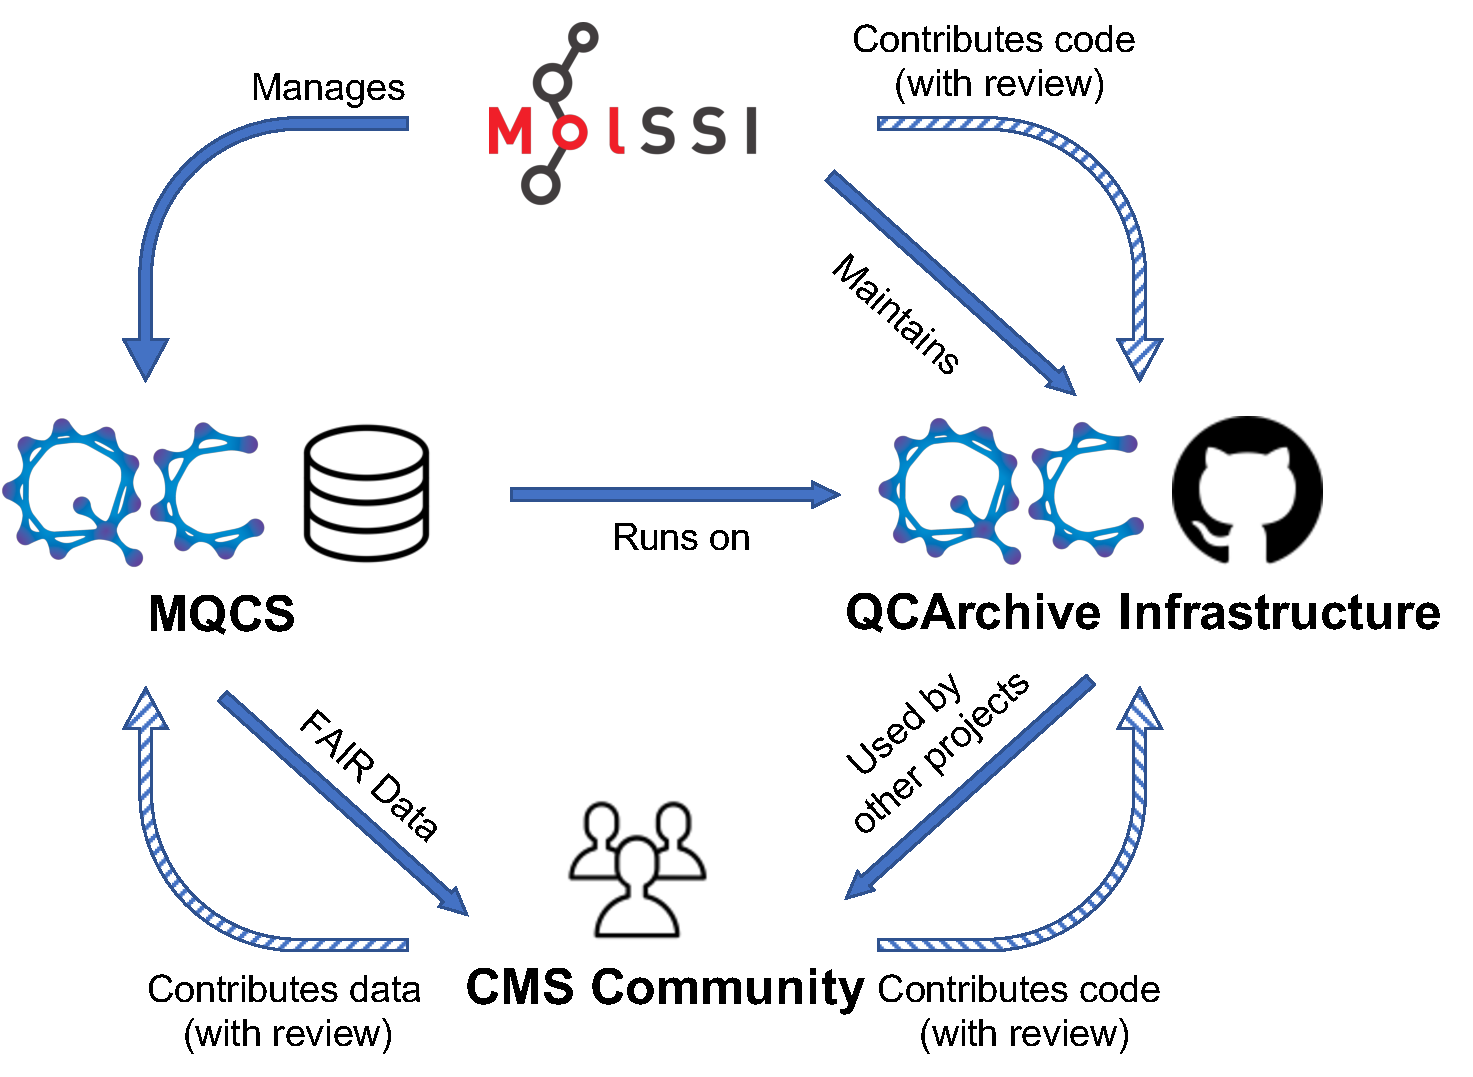
\includegraphics[width=\columnwidth]{images/community_model.pdf} % will be less gargantuan in two column format
    \caption{Relationship between the \qca project, MolSSI, and the CMS community.}
    \label{fig:community}
\end{figure}

The \mqcas can also be used by the community for those in collaboration with MolSSI and who have target data in mind.
In these instances, the community groups can submit new datasets and computations to the \mqcas but are required to supply physical resources to evaluate submitted computational tasks.
Several examples are the Open Force Field Initiative to expand data for force field fitting and ``A Collection of Chemistry DataBases'' (ACCDB)\cite{doi:10.1002/jcc.25761} who is assisting the expansion of literature datasets.
\textcolor{red}{Submitted datasets are reviewed by the \mqcas maintainers for integrity and often require comparisons
to literature values to ensure consistency before accepting a contribution.}
Expanding the community program is central to the long term goals of the \mqcas, and additional community groups are actively sought.

The software stack supporting the \mqcas, dubbed \qcai, is open-source and modular for reuse by the CMS community.
The \qcai can be used by individuals, single research groups, or multiple research groups depending on the data sharing targets of the groups in either public or private settings.
Private \qcai instances are fully as capable as \mqcas but are isolated from the public \mqcas and do not communicate until and unless the owner chooses to share their data.
The open-source \qcai is already used by a number of research groups that are unaffiliated with MolSSI and have now contributed back dozens of new software features that enhance the capabilities for all researchers using the infrastructure to simplify both their computation and data management.


\section{Infrastructure}

\subsection{Design goals}
\begin{itemize}
    \item {\it A modular platform.} Though it is often appealing to develop monolithic software to ensure integration between all components, we believe modular software promotes wider adoption in the open-source arena. This loose coupling allows each building block of the core infrastructure to be used in projects beyond the \qca scope.
    \item {\it Building on community software.} The \qca platform exists to promote and link, rather than replace, existing community software. This is evident in several building blocks which collectively wrap dozens of community-built codes and seek to add more through unified interfaces.
    \item {\it An open developer community.} All software developed by MolSSI exists on GitHub, where contributions, discussion, criticisms, and bug reports are encouraged and recorded for posterity.
    \item {\it Software practices.} The infrastructure follows MolSSI's software ``Best Practices''\cite{GH20:molssi-best-practices, GH20:molssi-cookiecutter} guidelines for contributing, layout, testing, and module distribution.
    \item {\it Software distribution.} The monthly release cycle is automatically deployed to PyPI\cite{GH20:pypi}, Conda\cite{GH20:conda}, and Docker\cite{GH20:docker} images to ensure ease of use in other projects. Examples of all software projects can also be automatically deployed via Binder\cite{project_jupyter-proc-scipy-2018} and Google Colab\cite{GH20:colab}.
\end{itemize}

\subsection{Software Components}

The \qcai software components unify to form a platform that can represent computations as structured data, automatically run those computations on a diverse set of physical resources, store computation results, and provide a Python-based front-end to submit and query computations.
In addition to forming a complete platform, the five software components were carefully constructed to be usable outside of the \qca stack to maximize community utility and reusability.
A brief overview of each component can be found below:

\begin{itemize}
    \item \qcel - Periodic table information, version-controlled physical constants, molecule parsing, testing infrastructure, and \qcsk models. \url{https://github.com/MolSSI/QCElemental}
    \item \qcng - Quantum chemistry and CMS community program executor with \qcsk enforced input/output models. \url{https://github.com/MolSSI/QCEngine}
    \item \qcf - Distributed task scheduler and executor, database store for chemistry results, and organization of results at scale. \url{https://github.com/MolSSI/QCFractal}
    \item \qcptl - Data querying, visualization, organization, and statistical analysis for chemistry-related results and a front-end client for \qcf. \url{https://github.com/MolSSI/QCPortal}
    \item \qcsk - A community built key-value/array description of QC (or QC-like) objects such as molecules and
input/output quantities from QC programs. \textcolor{red}{(This important component, which has been developed
somewhat separately from the rest of the \qca package, will be decscribed in a later publication.)} \url{https://github.com/MolSSI/QCSchema}
\end{itemize}



%\begin{itemize}
%    \item Provide a brief overview of the process by which \qca does its work. QCPortal talks to QCFractal which executes \qcngs on \qcsk, taken from \qcel, to generate output schema. This should be a brief introduction so as the reader is going through each component, they can reference back to this section/a figure to better understand its place in the work.
%    \item If we simply start discussing the components, the reader will have trouble placing things in the platform, so we want to first discuss the process of \qca so they can reference back to it and gain a better understanding.
%\end{itemize}

\subsubsection{\qcel}

\qcel encodes data layouts for fundamental CMS entities like Molecule, OptimizationResult, and BasisSet into object-oriented ``models'' that can be used in Python.
In addition to forming a Python reference implementation of the community-built \qcsk, the models impose validation to layout (e.g., $3 * N_{\text{atoms}}$ coordinates) and physics (protons $-$ electrons = charge) beyond what JSON Schema\cite{WEB20:jsonschema} (the implementation of \qcsk) can specify.
Models further define convenience functions like Molecule string parsing, coordinate alignment, and structure measurement.
The serialization of models is automatic and transparent, including binary/JSON and shaped/flat array data, and recursively extends to all hierarchical models.
By embellishing the base \qcsk data layout, \qcel can avert much of the serialization, translation, resizing, and validation code that inevitably surrounds every downstream \qcsk implementation.
This focuses community discussion on the implicit contracts for \qcsk transactions that JSON Schema cannot define and provides modular building blocks for CMS applications.

\qcel also collects metadata vital to reproducibility in CMS that are difficult to find in structured format (often websites or journal tables) and that are being continuously refined, namely physical constants, periodic table metadata (masses, common isotopes, etc.), covalent radii, etc.
These collections are placed behind a light Python API, labeled by context (e.g., CODATA2018), and backed by unit conversion tools. \qcel can thus facilitate migration of community software toward modern and consistent values, while ensuring that with a context switch, conversions to older data are reproducible.
\qcsk values are stored in atomic units to minimize susceptibility to such details and the \qcel arbitrary unit conversion is used to support the diverse fields and units CMS codes demand.
A small \qcel example can be seen in Fig.~\ref{fig:qcelemental}.

\begin{figure}[H]
    \centering
    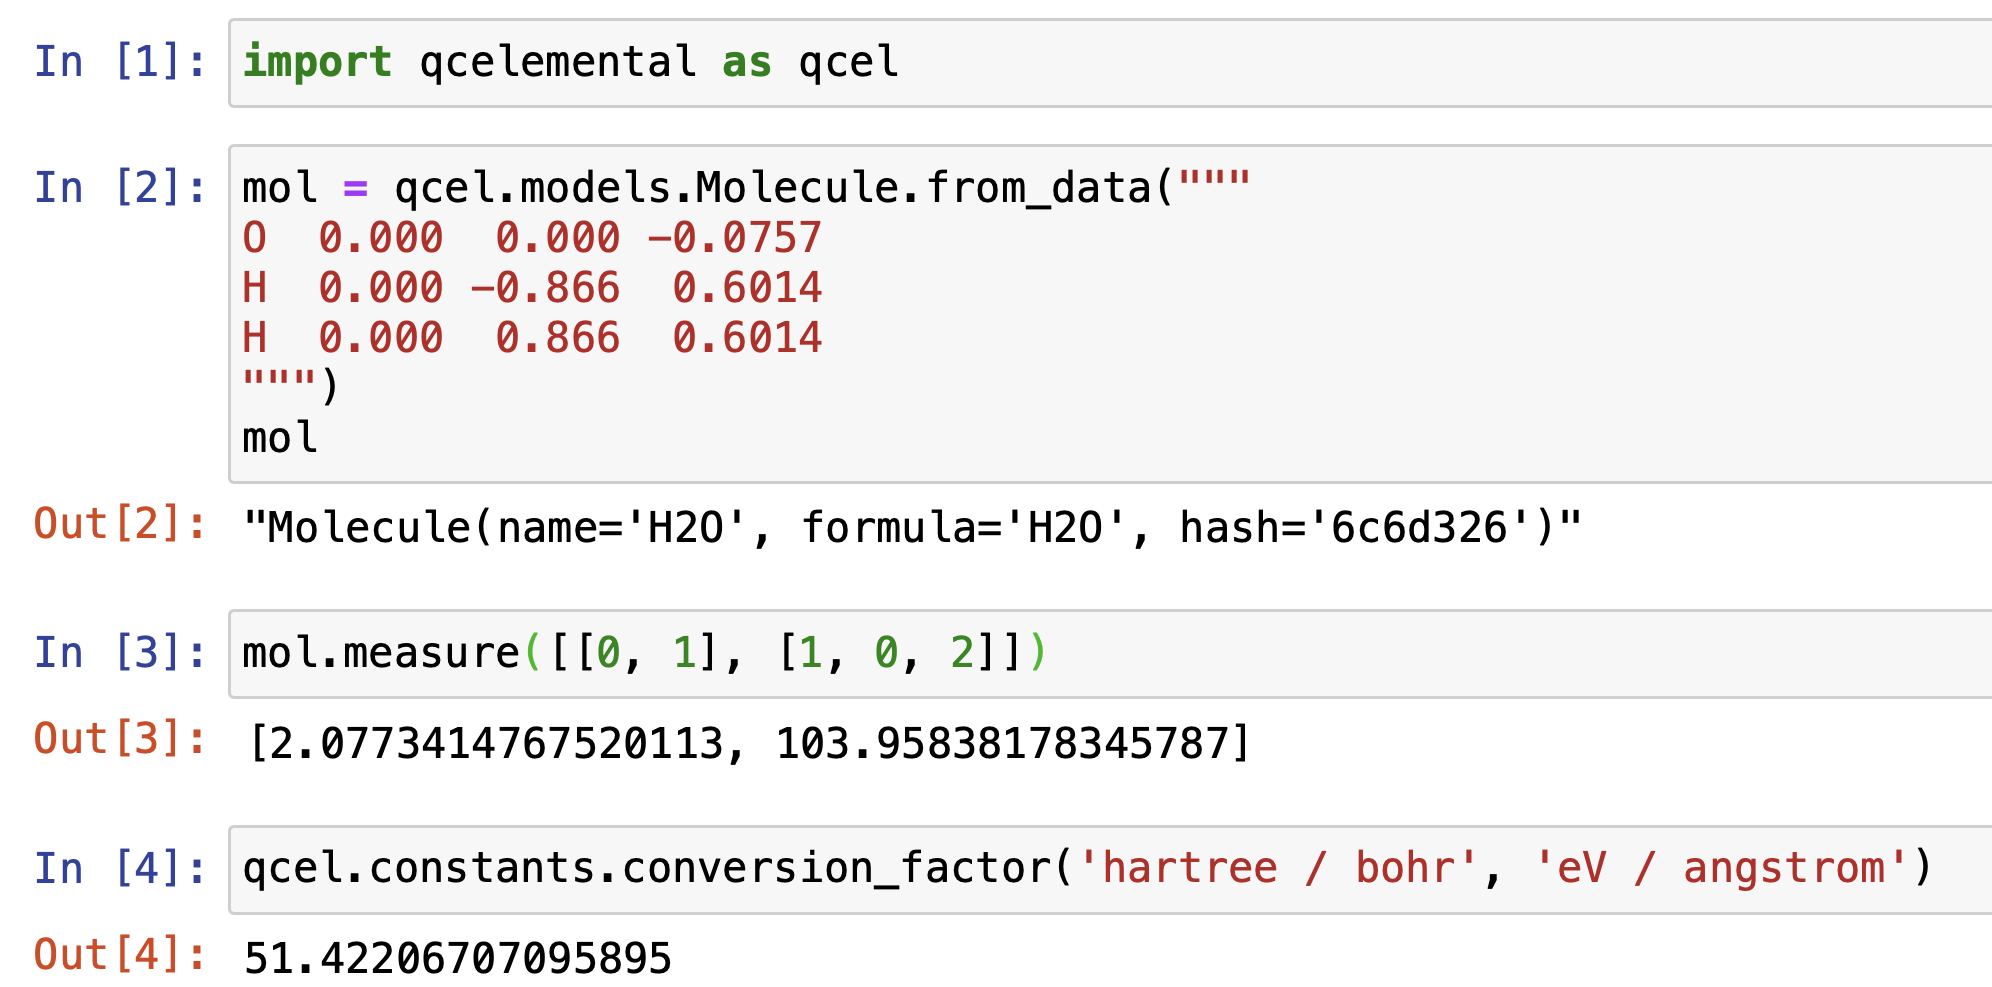
\includegraphics[width=\columnwidth]{./images/QCElementalImage.png}
    \caption{A Jupyter notebook showing a Molecule object created from an XYZ string, the O-H distance (Bohr) and H-O-H angle (degrees) measured, and the computation of a conversion factor for a gradient.}
    \label{fig:qcelemental}
\end{figure}

\subsubsection{\qcng}

\qcng is a unified function-based execution engine that provides \qcsk input and output objects for a variety of programs.
\qcng provides this uniform input/output for any program which can be expressed within the restraints of the schema and, as such, covers a variety of quantum chemistry, semi-empirical, force field, and machine learning inference programs.
\qcng works by either interfacing with a program directly at the Python layer or translating the domain-specific input file that a program expects and parsing the subsequent log file or, if available, structured output files.
The execution layer automatically discovers the locations and versions of available programs, configures them based on physical resource constraints such as memory and number of physical cores, and isolates and cleans up scratch directories.

The persistent use of \qcsk descriptions in \qcng simplifies writing software that uses CMS programs.
The input to all computations is a \qcsk specification document, such as an \texttt{AtomicInput} describing standard input to atomistic calculations (e.g., gradient evaluations).
Very few aspects of the inputs to \qcng are tied to the actual code which will fulfill the specified calculation, allowing users to efficiently perform computations with different quantum chemistry codes as scientific demands change.
The output from the codes is also returned in a standardized form, which simplifies databases and any software to analyze the outputs of a QC program.
Two examples: 1) a Hessian computed with Psi4\cite{Parrish:2017:3185} and NWChem\cite{Valiev:2010:1477} can be analyzed with the same software and
2) the geomeTRIC optimization package\cite{ping2016geometric, GH20:geometric} uses \qcng as an interface to different quantum chemistry packages so as to be agnostic the backend program.

\qcng also automatically gathers information needed to reproduce calculations. 
The input \qcsk  completely specifies and documents the calculation that was performed, and the \qcng executable records all required outputs.
All computations that are evaluated with \qcng return provenance information including program version, hardware specification, physical resources utilized, and \qcng version.
Tracking this information provides both reproducibility and history of every computation undertaken with this software platform.
The inputs, provenance, and outputs of a calculation are all stored in the same document, which makes it less likely that metadata will be lost.

Currently the following programs are interfaced to \qcng:

\begin{itemize}
     \item {\it Quantum Chemistry}:
     CFOUR,\cite{WEB19:cfour}
     Entos,\cite{Manby:2019:entos} 
     GAMESS,\cite{GAMESS:2005}
     Molpro,\cite{WEB20:molpro,MOLPRO-WIREs}
     NWChem,\cite{Valiev:2010:1477}
     Psi4,\cite{Parrish:2017:3185}
     Q-Chem,\cite{Shao:2015:184}
     Terachem,\cite{Ufimtsev:2009:2619}
     Turbomole\cite{Furche:2014:91}
     \item {\it Semi-empirical}:
     MOPAC\cite{WEB20:mopac}
     \item {\it ML Potential}:
     TorchANI\cite{GH20:torchani, Smith:2017:3192}
     \item {\it Molecular Mechanics}:
     RDKit,\cite{GH20:rdkit}
     OpenMM\cite{Eastman:2017:1}
     \item {\it Analytical Corrections}:
     DFTD3,\cite{GH20:dftd3, Grimme:2010:154104}
     MP2D\cite{GH20:mp2d, Rezac:2018:4711}
     \item {\it Geometry Optimizers}:
     geomeTRIC,\cite{GH20:geometric, Wang:2016:214108}
     PyBerny\cite{GH20:pyberny}
\end{itemize}

Interfacing to additional programs is an ongoing effort that is open to community contributions and suggestions.
Many of the wrappers for specific software has been contributed by non-core \qcng developers, such as Entos, Molpro and MOPAC.
A short example computation can be found in Fig.~\ref{fig:qcengine}.

\begin{figure}[H]
    \centering
    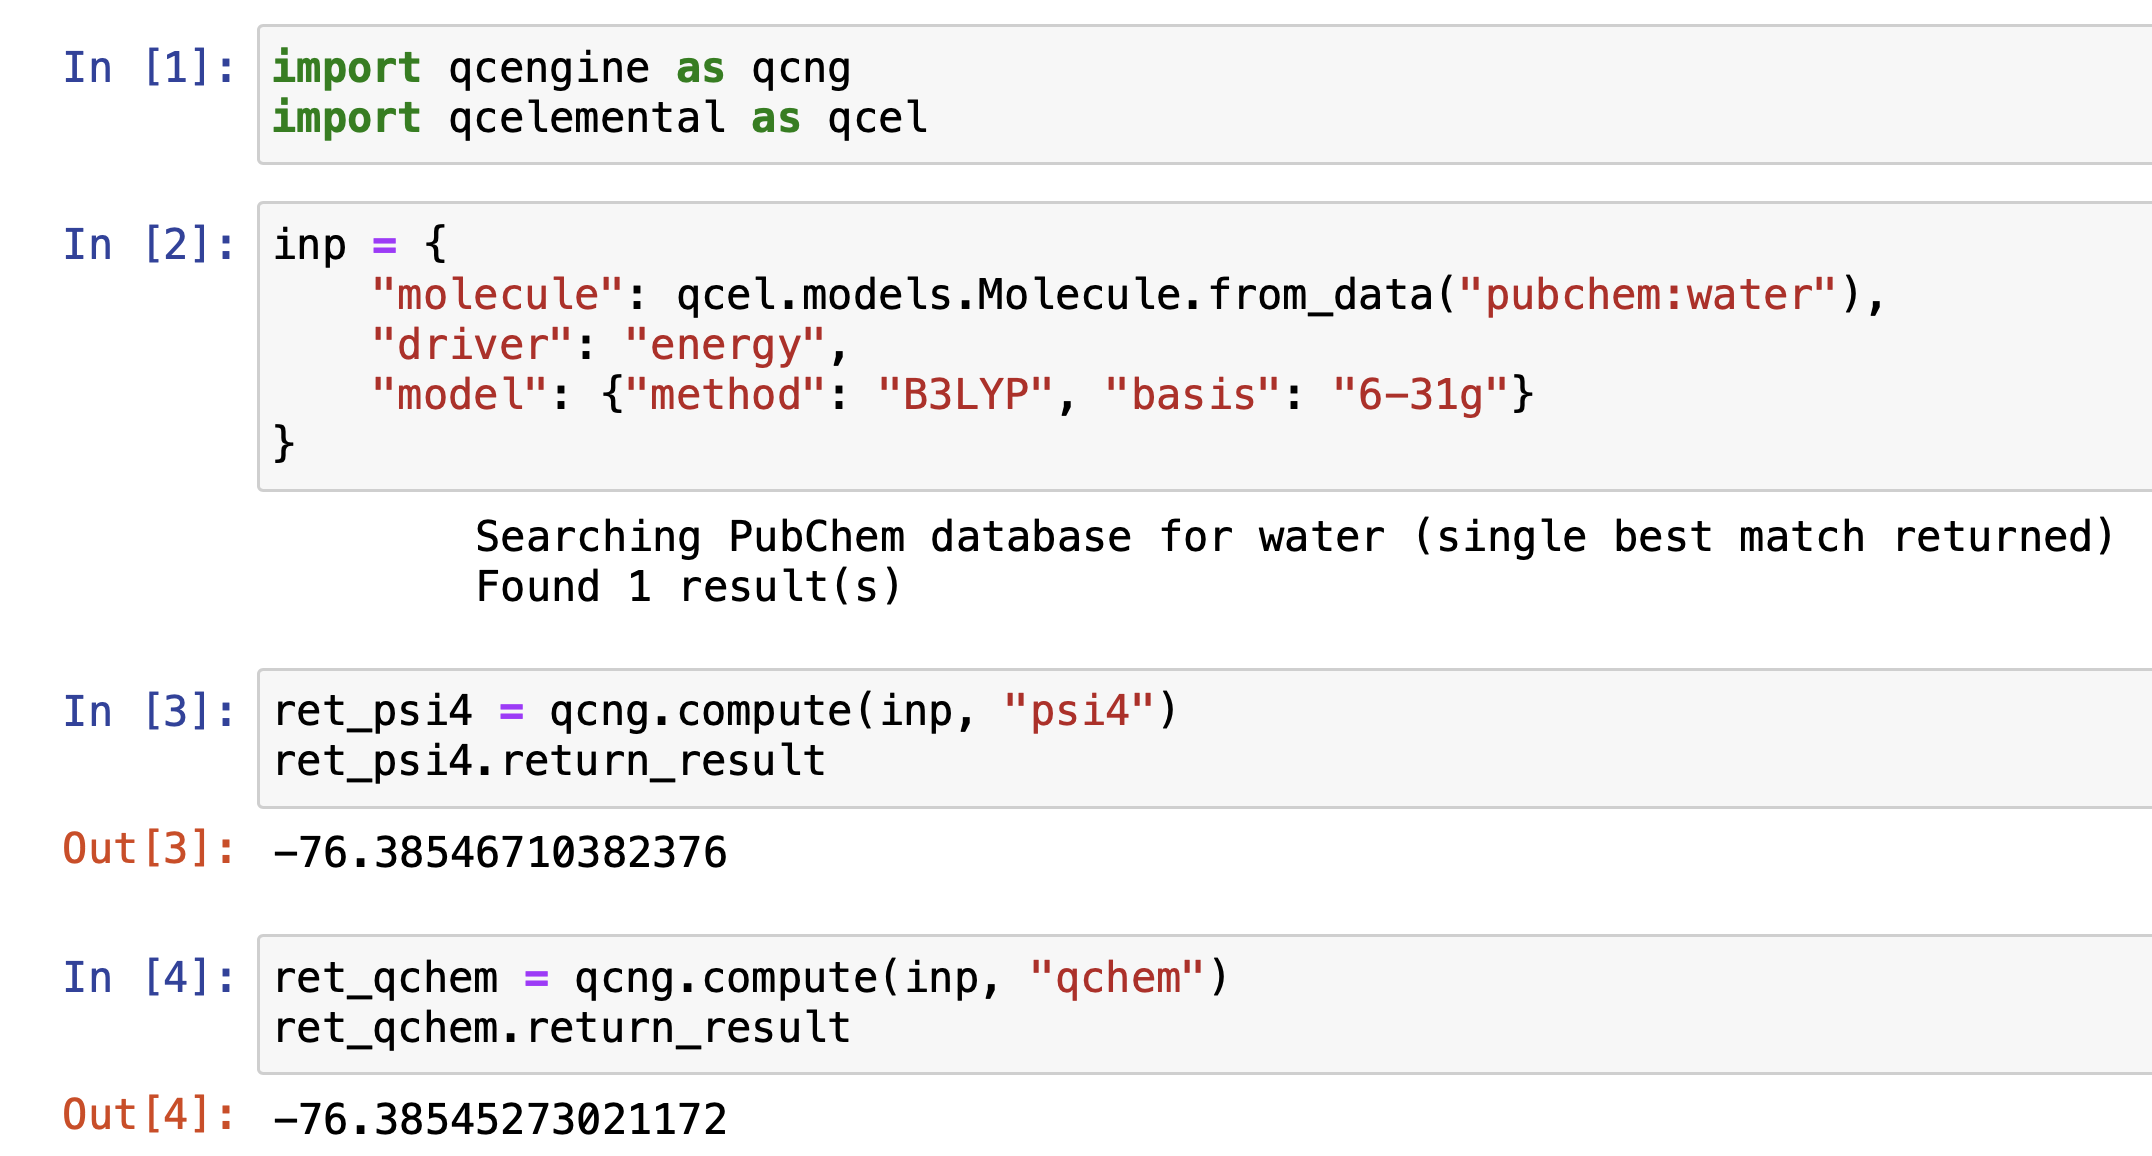
\includegraphics[width=\columnwidth]{./images/QCEngineImage.png}
    \caption{A Jupyter notebook demonstrating pulling a water geometry from the PubChem database\cite{10.1093/nar/gky1033} and computing both Q-Chem and Psi4 with the same input. Note the difference in absolute energies is primarily due to the fact that Q-Chem uses direct SCF algorithms by default while Psi4 uses density-fitting.}
    \label{fig:qcengine}
\end{figure}

\subsubsection{QCFractal}

\qcf is the central server of the \qca platform, providing distributed computing, data storage, and data querying capabilities.
Fundamentally \qcf is a campaign manager designed for long-duration (years) deployments to passively manage all
computation and data storage requirements for an individual researcher or groups of researchers concurrently. 
For reference, the \mqcas has currently run for eight months without issue, serves data to over a thousand unique users per month, and evaluates 1--5M tasks per month.
It is estimated that the \mqcas has the projected capacity to scale by at least 15 fold without optimization.

Storage of computations and associated metadata is accomplished by using a SQL relational database (PostgreSQL\cite{WEB20:postgres}).
The SQL database is structured so that each type of \qcel object stored (\texttt{Molecule}, \texttt{AtomicResult}, etc.) has its own table in the database, and composite objects like \texttt{AtomicResult}, which contain a \texttt{Molecule} object internally, reference the required table instead of storing the object.
For example, a single \texttt{Molecule} object can be related to many different energy or gradient calculations so that the molecule is not duplicated, saving space, and all computations related to the molecule can be quickly queried.
Each stored object has a carefully constructed unique identifier that can be computed from the object itself.
The unique identifier makes it trivial to identify duplicate records and prevent the same calculation from being run twice.
\textcolor{red}{For example, unique identifiers for given single point computation are molecule, method, basis,
program, and keyword arguments create a unique computation.}
If a computation with the same molecule is requested by another computation, each computation links to the same molecule in the database.
This linking structure makes tedious composite computations of multiple molecular properties effortless.

To evaluate tasks, \qcf provides a central task queue, which can be evaluated by a single or many ``managers'' who interface with a physical resource (campus cluster, supercomputer, cloud resource, or workstation).
Each manager can consume either the entire or a fraction of the physical resource, depending on configuration, through a unified cluster interface.
Mangers use existing task execution systems like Dask\cite{matthew_rocklin-proc-scipy-2015}, Parsl\cite{babuji19parsl}, RADICAL\cite{10.1109/CCGRID.2018.00051}, and Fireworks\cite{CPE:CPE3505} to accomplish high-throughput distributed computing within a given resource, leveraging large amounts of software infrastructure work by the community.
In particular, for traditional HPC resources, these task execution systems hook into queuing systems like SLURM\cite{10.1007/10968987_3} to submit ``workers'' to nodes, which in turn evaluate tasks.
Each of these execution systems eliminates the need for humans to submit each computation to the queuing system.
The managers stay resident on the system and can automatically remove or request new resources depending on the number of tasks in the central task queue.
A diagram of a task execution system is given in Fig~\ref{fig:infrastructure}.
The end result is that users submit tasks through a single interface, and the tasks are automatically evaluated on any physical resource to which the user has access.

\qcf can also run workflow ``services'' to orchestrate sophisticated computational campaigns built out of interdependent tasks.
For example, a TorsionDrive\cite{torsiondrive} service will compute the energy surface of a molecule at a frozen set of dihedral coordinates.
The TorsionDrive program is a standalone open-source package\cite{WEB20:torsiondrive} that implements an iterative procedure for computing smooth dihedral scans.
At each step in the iterative TorsionDrive service, new geometry optimizations are supplied by the TorsionDrive package and placed into \qcf's central task queue.
Once all computations for each iteration are complete, \qcf uses the TorsionDrive package to discover the starting geometries of the next round of geometry optimizations.
The TorsionDrive service is iterated until the entire dihedral scan has been completed, and a smooth energy profile has been achieved.
The \mqcas routinely iterates thousands of services like TorsionDrive concurrently to completely saturate available computational resources.

In addition to the TorsionDrive service, a GridOptimization service that can do multi dimensional scans of bonds, angles, and dihedrals combined is also implemented.
Many future services are in development such as automated conformational searches, reaction pathways, finite difference gradients and Hessians, and more.
A core feature of the services is that they can import the logic of different programs and request standard building blocks such as energy and geometry optimizations from the central task queue.

\begin{figure}[H]
    \centering
    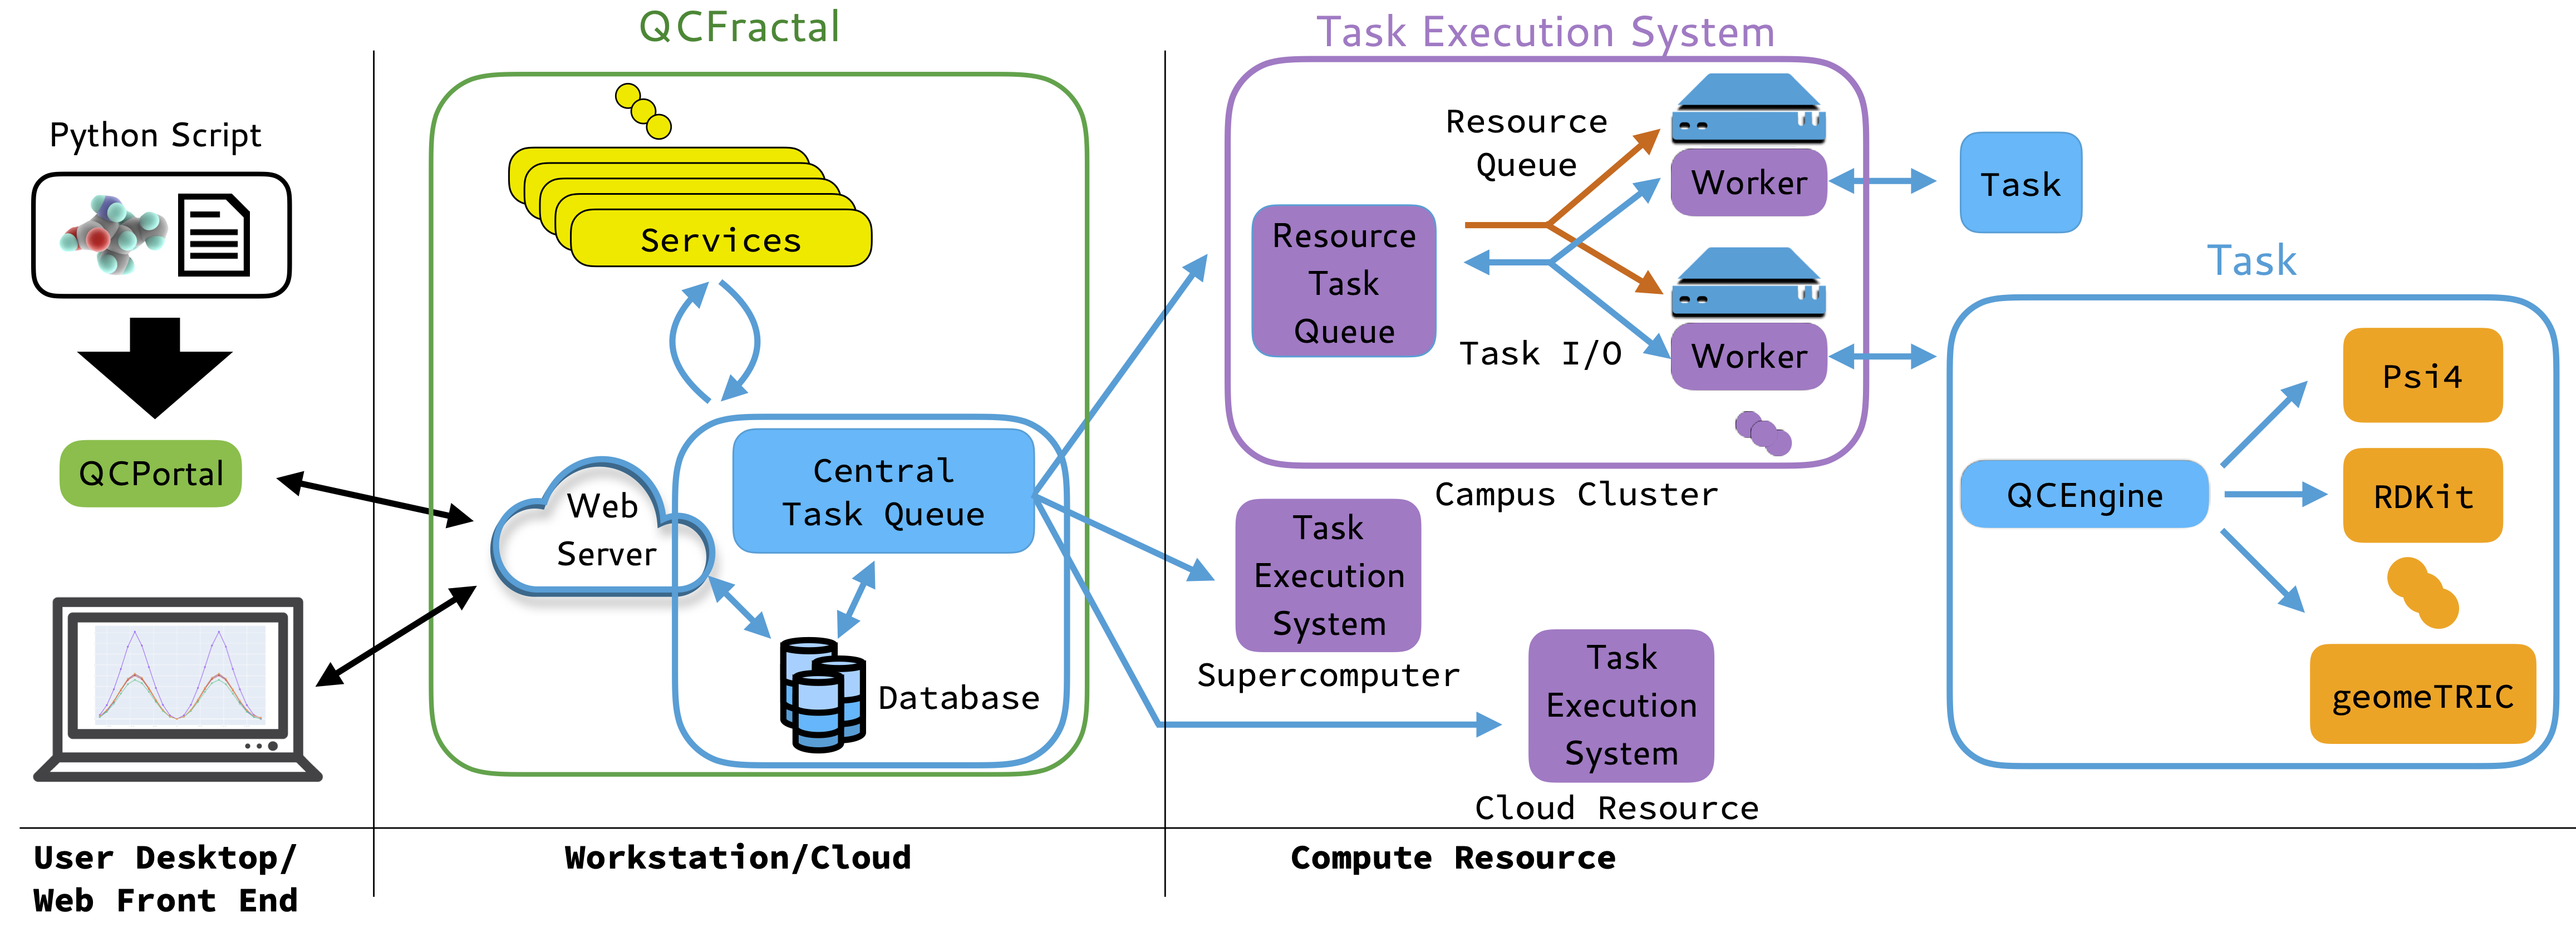
\includegraphics[width=\columnwidth]{./images/QCArchiveLayout.png}
    \caption{The full \qcai and how each layer and module communicates. Between different locations, all pieces communicate over TCP/IP protocols; within individual boxes, all pieces are connected through a single Python interpreter; and between a resource task queue and workers, communication can come in a variety of RPC sockets over either MPI or local Ethernet.}
    \label{fig:infrastructure}
\end{figure}

\subsubsection{QCPortal}

\qcptl is a front-end client for \qcf that is able to access data from the server in a user-friendly fashion and spawn new compute tasks to be evaluated.
The basic organizational unit of \qcptl is the collection, a grouping of computations into commonly usable forms.
For example, the ``Dataset'' collection is a dataframe (two-dimensional tabular data) with rows corresponding to named Molecules and columns corresponding to a model chemistry (e.g., B3LYP-D3/def2-SVP).
The cells in the dataframe reference individual computations in the \qcf database.
New molecules or model chemistries can be added to a Dataset at any time and will be tracked by the Dataset for future use.
Data handling is supported by the popular Pandas\cite{mckinney-proc-scipy-2010} library for manipulating dataframe objects.

Interactive Python sessions such as Jupyter\cite{Kluyver:2016aa} and Google Colab\cite{GH20:colab} are core features of \qcptl allowing real-time manipulation of data, visualization of common properties, and built-in charts and properties.
This includes visualization capabilities for \texttt{Molecule} objects (supported by NGLView\cite{10.1093/bioinformatics/btx789}), automated performance characteristics of methods computed on Datasets, and graphs that demonstrate the energy profile of a geometry optimization per step.


\begin{figure}[H]
    \centering
    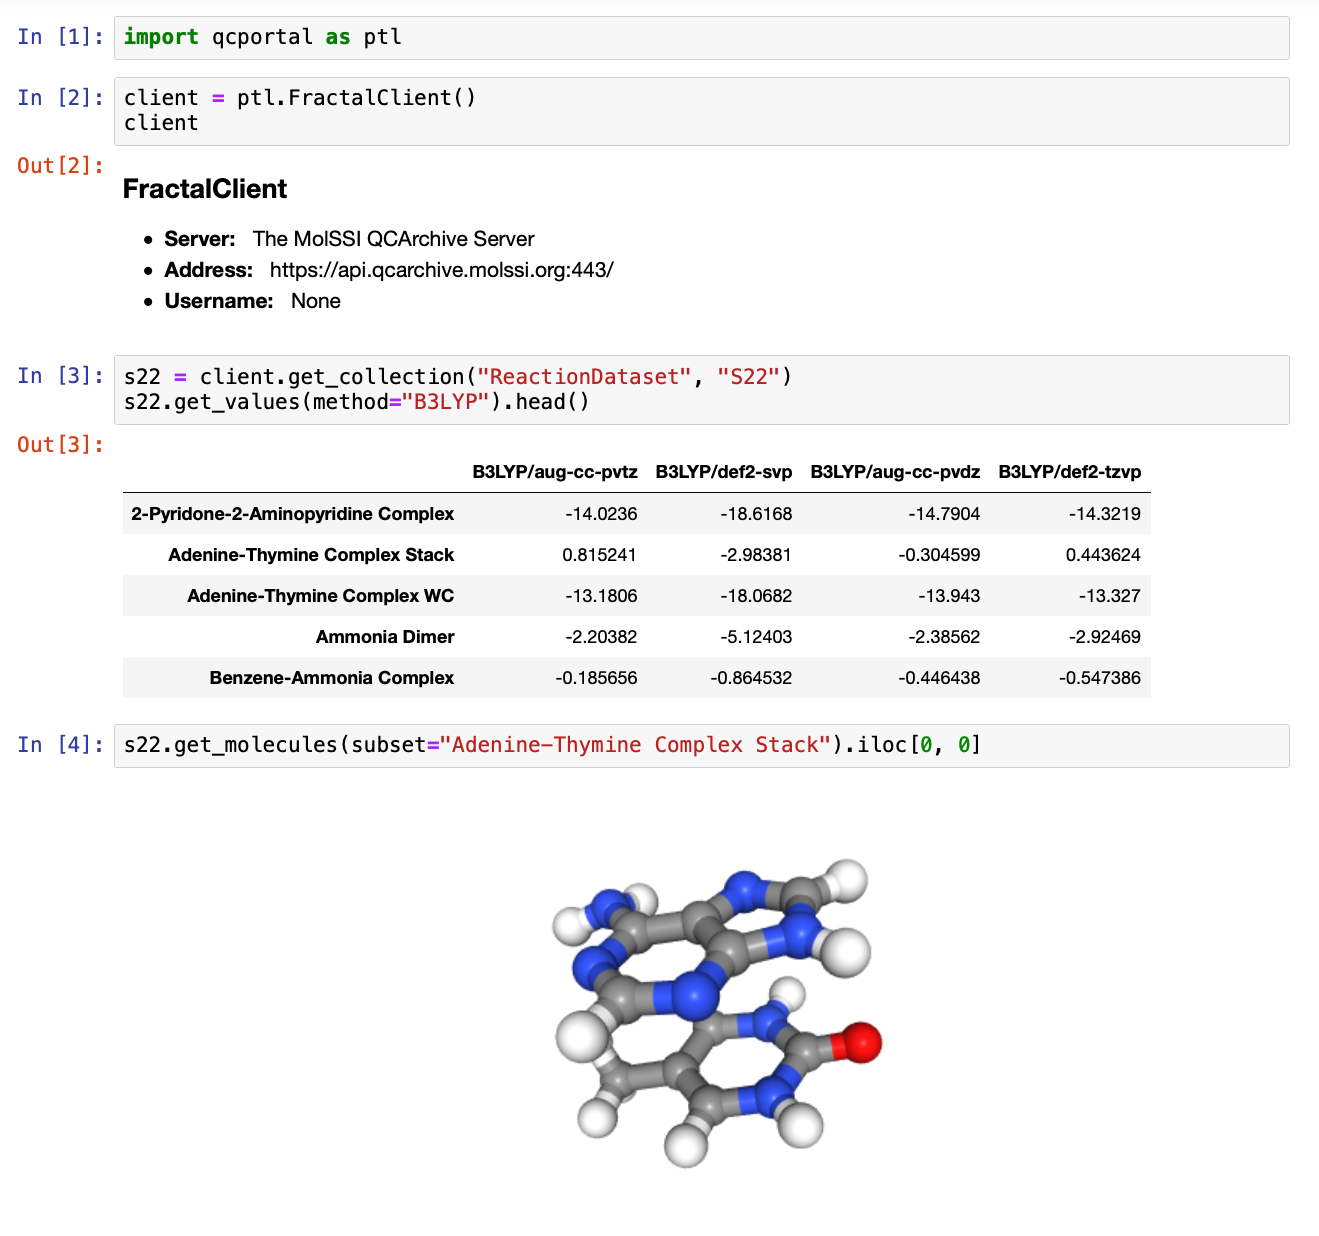
\includegraphics[width=\columnwidth]{./images/QCPortalImage.png}
    \caption{An image showing \qcptl pulling the S22 Dataset from the \mqcas, listing all current B3LYP interaction energies, and rendering an example molecular complex from the dataset.}
    \label{fig:qcportal}
\end{figure}


\subsection{Examples}
A full software stack example is provided in the form of a TorsionDriveDataset, which computes TorsionDrives for different molecules at multiple levels of theory.
Computation with \qcf Datasets typically happens in three stages: 1) defining the molecules and relevant metadata (e.g., the dihedral angle to scan) in the Dataset, 2) the addition of computation specifications for evaluation, and 3) querying of the data during or after the computations have completed.

For the first stage, a \qcf client object is created that connects to a \qcf server on the internet. In this example, the \qcf server is on the same computer as the Jupyter Notebook.
A new TorsionDriveDataset is then created with the name ``TD Demo'', and, once created, this Dataset is permanently in the server unless explicitly deleted.
Next, hydrogen peroxide and butane geometries are pulled from \qcptl's small library of testing molecules. In general, molecules can be generated and imported from half a dozen common file formats.
Molecules are added with an alias for later reference along with the zero-index dihedral specification and the granularity of the torsion angle scan grid in degrees (Fig.~\ref{fig:torsiondrive1}).

\begin{figure}[H]
    \centering
    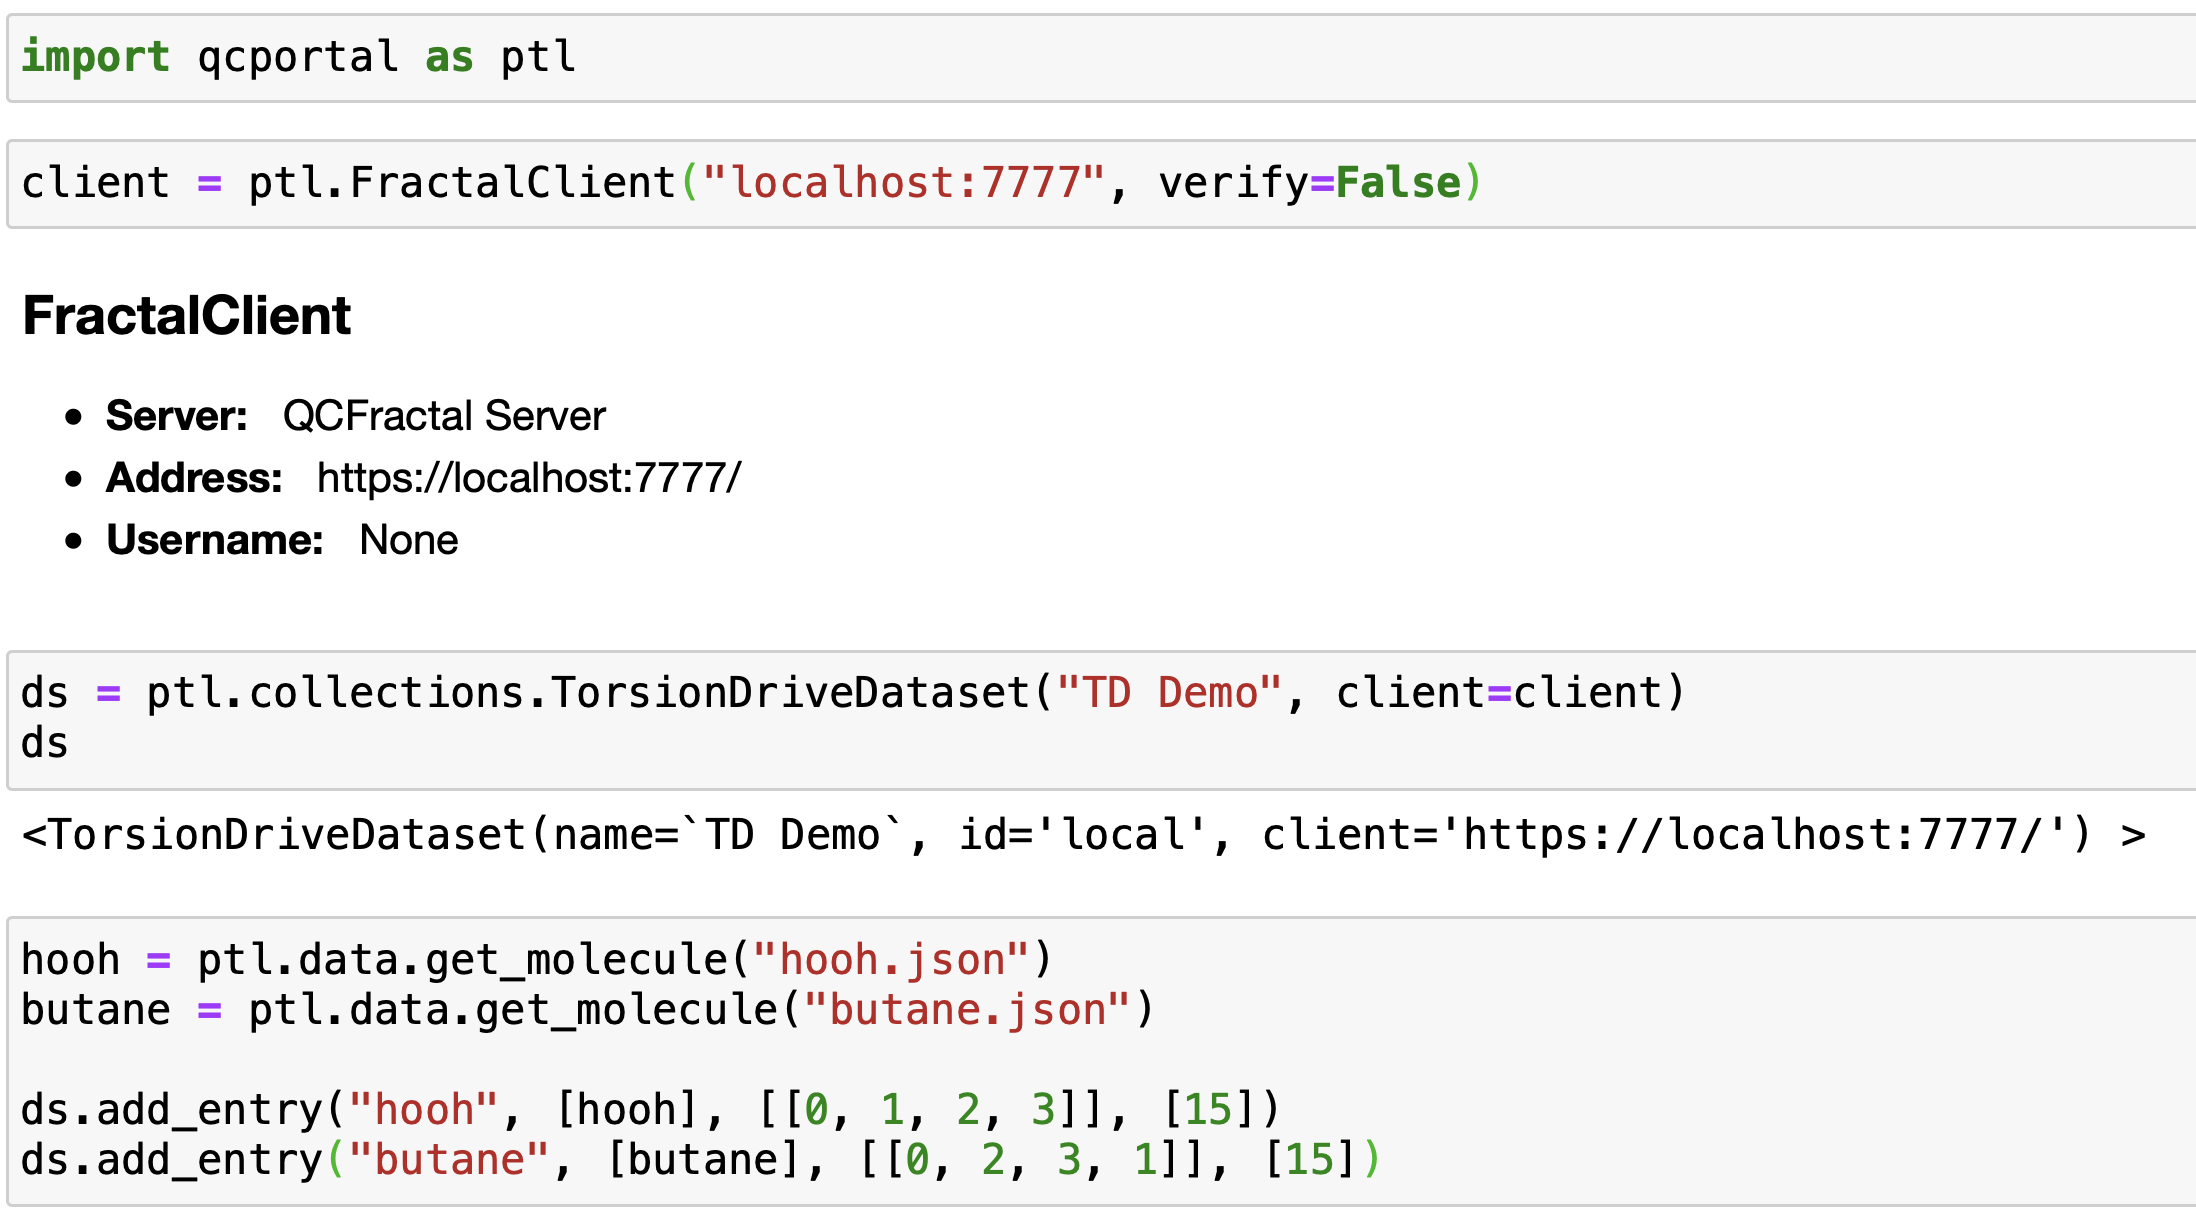
\includegraphics[width=\columnwidth]{./images/Example1.png}
    \caption{Setup of a new Dataset object.}
    \label{fig:torsiondrive1}
\end{figure}

The second stage involves the specification of the level of theory for each
TorsionDrive computation.  To provide a diverse example, a force field
(MMFF94~\cite{halgren1996merck}), machine-learned potential
(ANI-1x~\cite{smith2018less}), and a quantum chemistry level of theory
(B3LYP-D3(BJ)/def2-SVP~\cite{Becke93,Lee88:LYP,weigend2005a})
are chosen.  For each specification, the geometry optimization program,
method, basis set (optionally), and gradient evaluation program are also
chosen. Finally, calculations are submitted to the \qcf server's queue
(Fig.~\ref{fig:torsiondrive2}).

\begin{figure}[H]
    \centering
    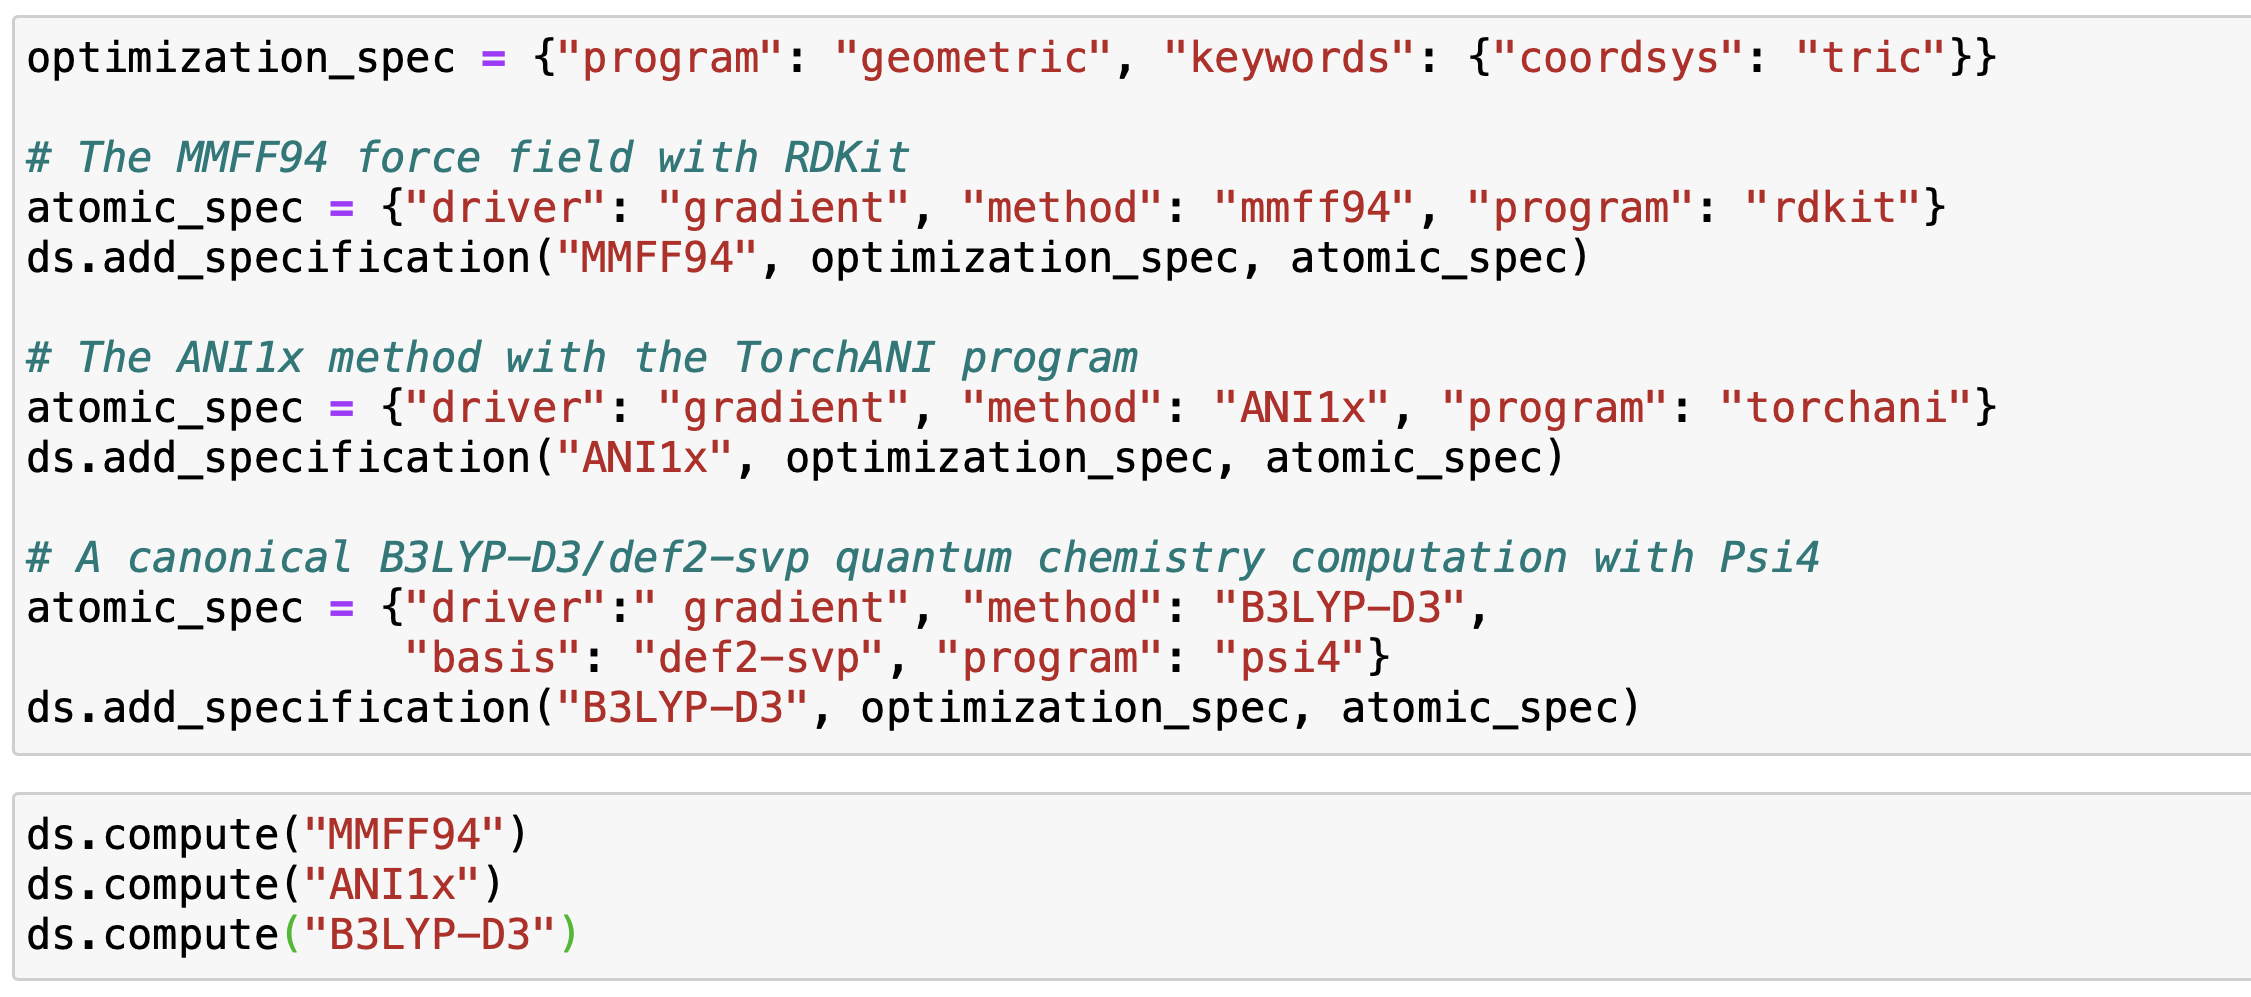
\includegraphics[width=\columnwidth]{./images/Example2.png}
    \caption{Computation on a Dataset object.}
    \label{fig:torsiondrive2}
\end{figure}

The final stage assumes that sufficient time has passed to evaluate the requested computations.
The researcher can then pull the TorsionDriveDataset from the server and begin to explore the results.
Shown is a simple example plotting the relative energy as a function of the dihedral angle for butane (Fig.~\ref{fig:torsiondrive3}).
In addition to the plot, every geometry optimization, molecule, gradient evaluation, logfile, and other computational detail can be queried and analyzed.

\begin{figure}[H]
    \centering
    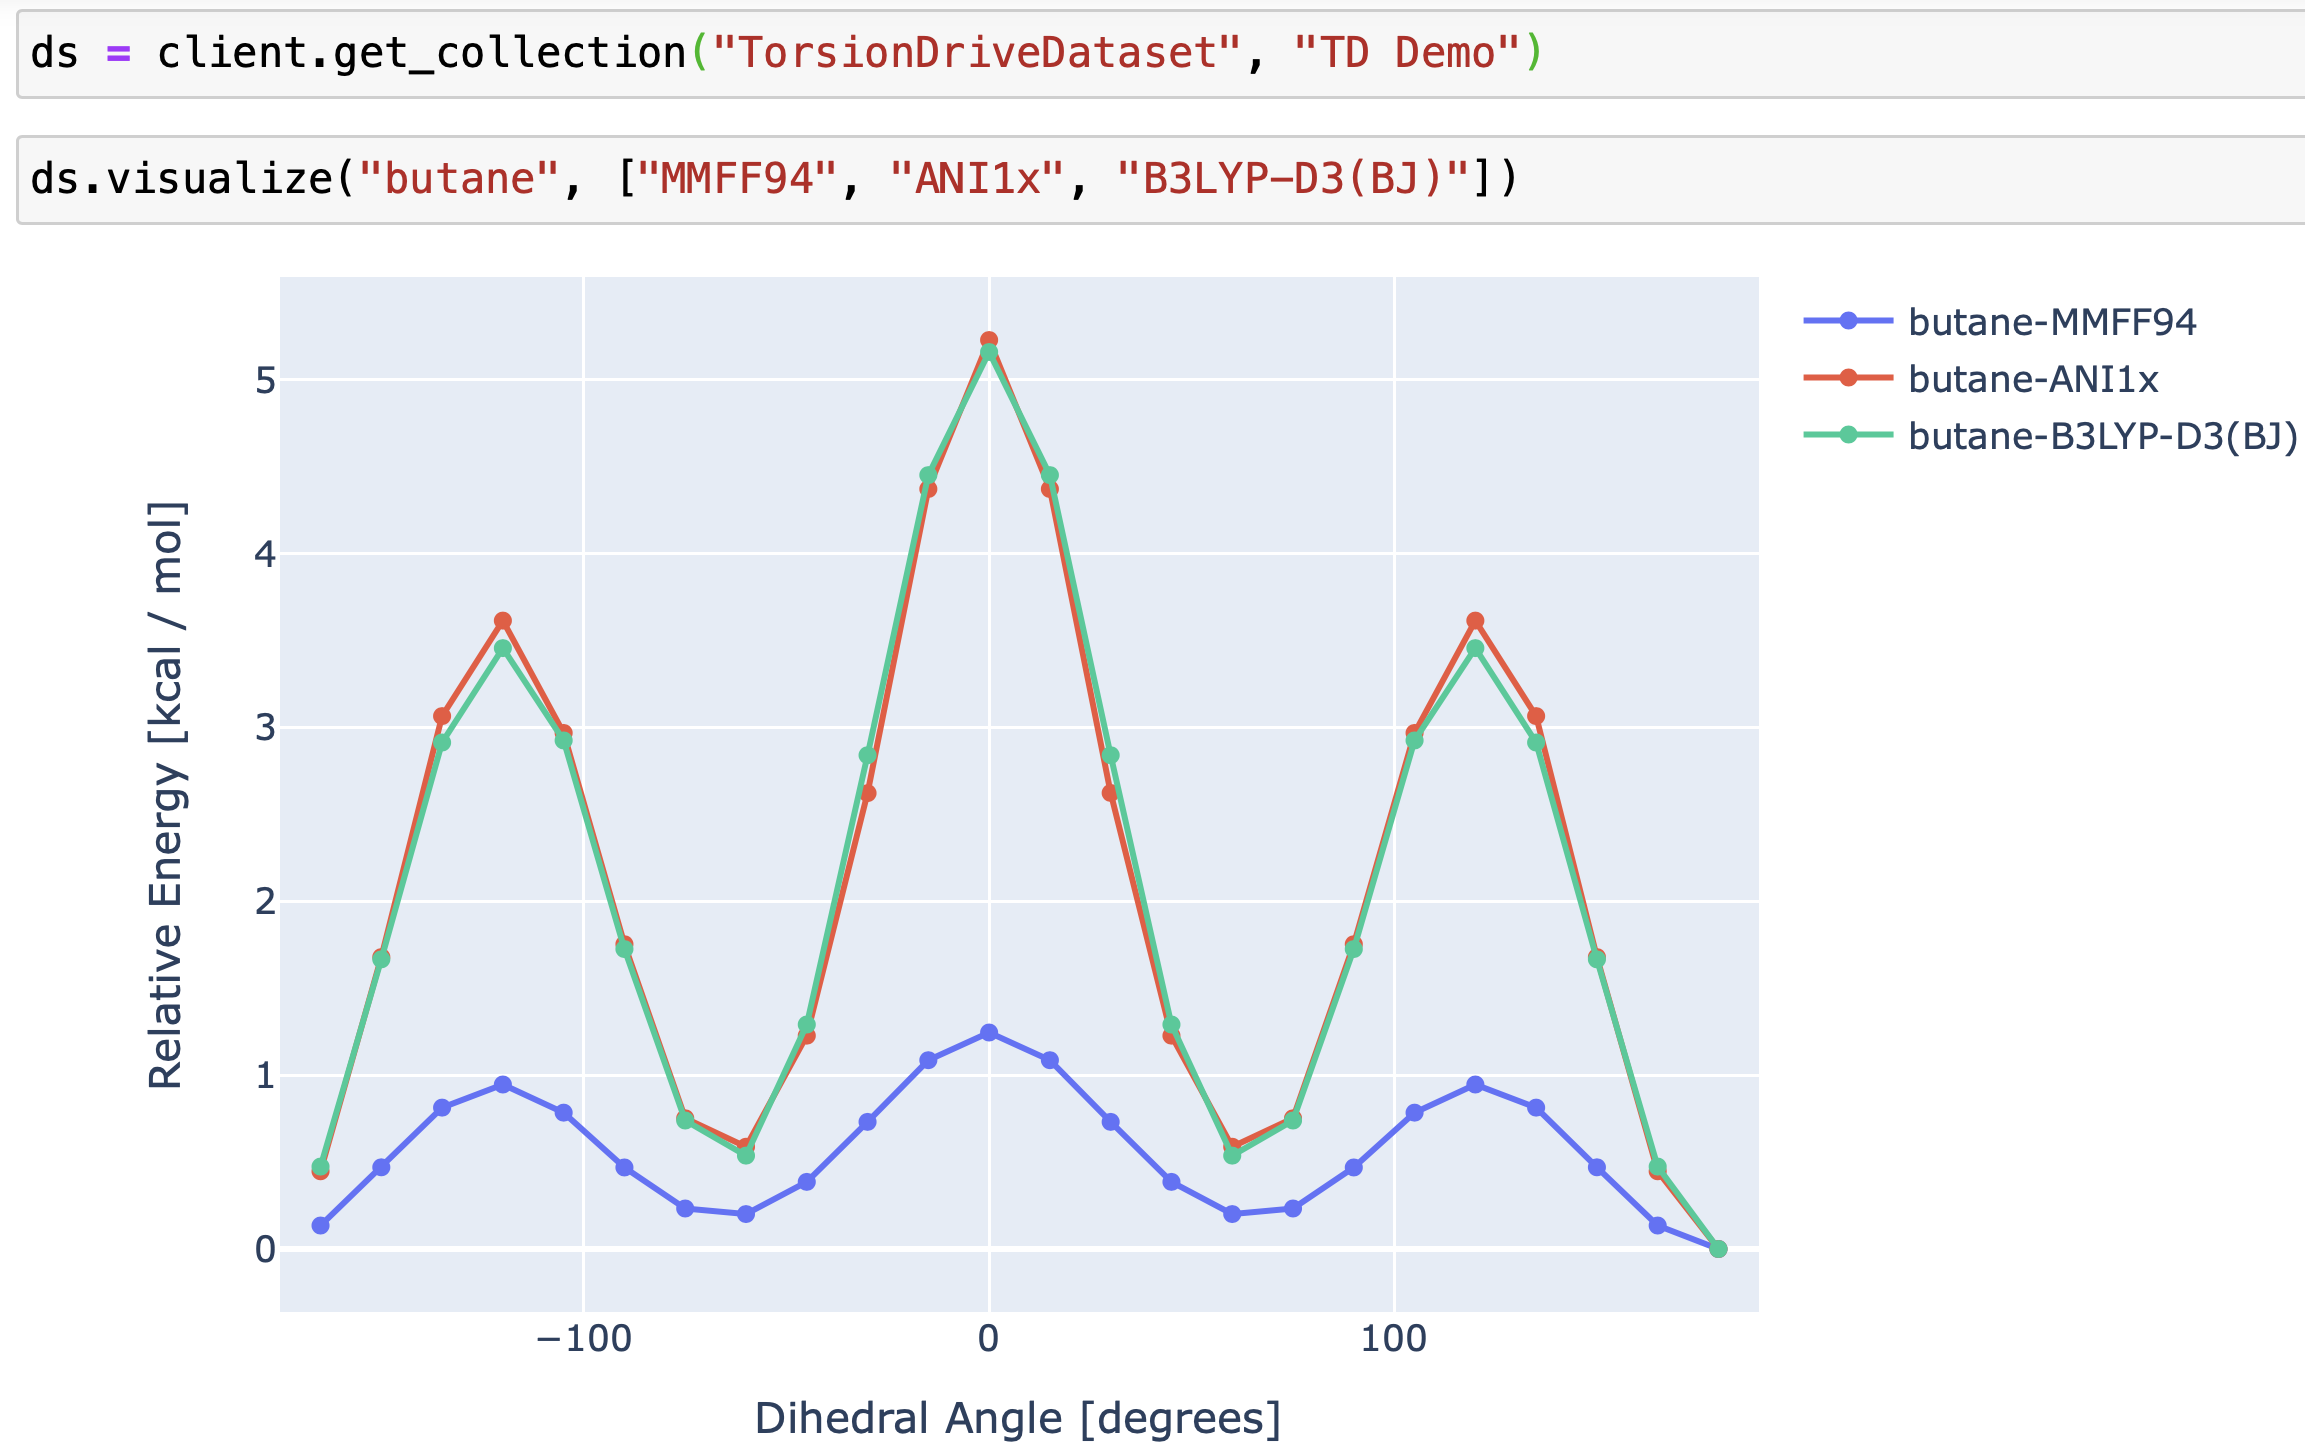
\includegraphics[width=\columnwidth]{./images/Example3.png}
    \caption{Visualization of a dataset object.}
    \label{fig:torsiondrive3}
\end{figure}

Large datasets in the \mqcas can contain hundreds of thousands of molecules (rows) and hundreds of computational methods (columns).
\textcolor{red}{A \qcf quick start guide to reproduce the above example can be found on our website
\cite{QCFractal:Quickstart}.}

\section{Web Applications}

To broaden the accessibility of CMS data beyond Python and Jupyter users, the \qca also provides access to its data through Web applications (Web apps).
Web apps serve users at all levels, from novice undergraduate students to the most advanced researchers and companies.
The goal is for users to view and explore data from the \mqcas in a facile but powerful way, making quantum chemistry available for general computational molecular scientists for a variety of use cases.

Each app is developed as a separate Flask-based\cite{WEB20:flask} micro-service with all apps available through the main \qca Web portal (\url{https://qcarchive.molssi.org}).
This approach enables easy extension and addition of new apps and potential contributions from the community to develop more apps.
\textsc{Plotly Dash}\cite{WEB20:dash} is used to compose web apps without requiring the use of Javascript, simplifying the process of hosting and creating new web applications.
The downside to \textsc{Dash} is that fine-tune control over the web app is lost and missing features require a more complex implementation making it  unsuitable for every web app. 

Currently, the \qca portal includes two apps, and more are under development with partners like the Science Gateways Community Institute\cite{SGCI} to work on the interactive app needs of the community. A brief description of current Web apps follows.


\subsection{Machine Learning Datasets Web App\label{sec:mlapp}}

The MolSSI Quantum Chemistry Machine Learning (ML) datasets repository provides a web app front-end to the curated ML datasets in the \mqcas.
These currently number 20, including ANI-1,\cite{Smith:2017:3192, Smith:2017:170193}
PC-9,\cite{Nakata:2017:1300, Glavatskikh:2019:69} and
ISO-17,\cite{Ramakrishnan:2014:140022, Schutt:2017:13890, Schutt:2017:991} and more are continuously added.
Datasets are ingested into a common format of structured metadata and are available for download in text format, or in structured HDF5 format.
Figure~\ref{fig:apps_ml_datasets} shows a screenshot of the ML datasets repository. 
All relevant citation information is shown to ensure the credit to the original authors is correctly assigned.

\begin{figure}[H]
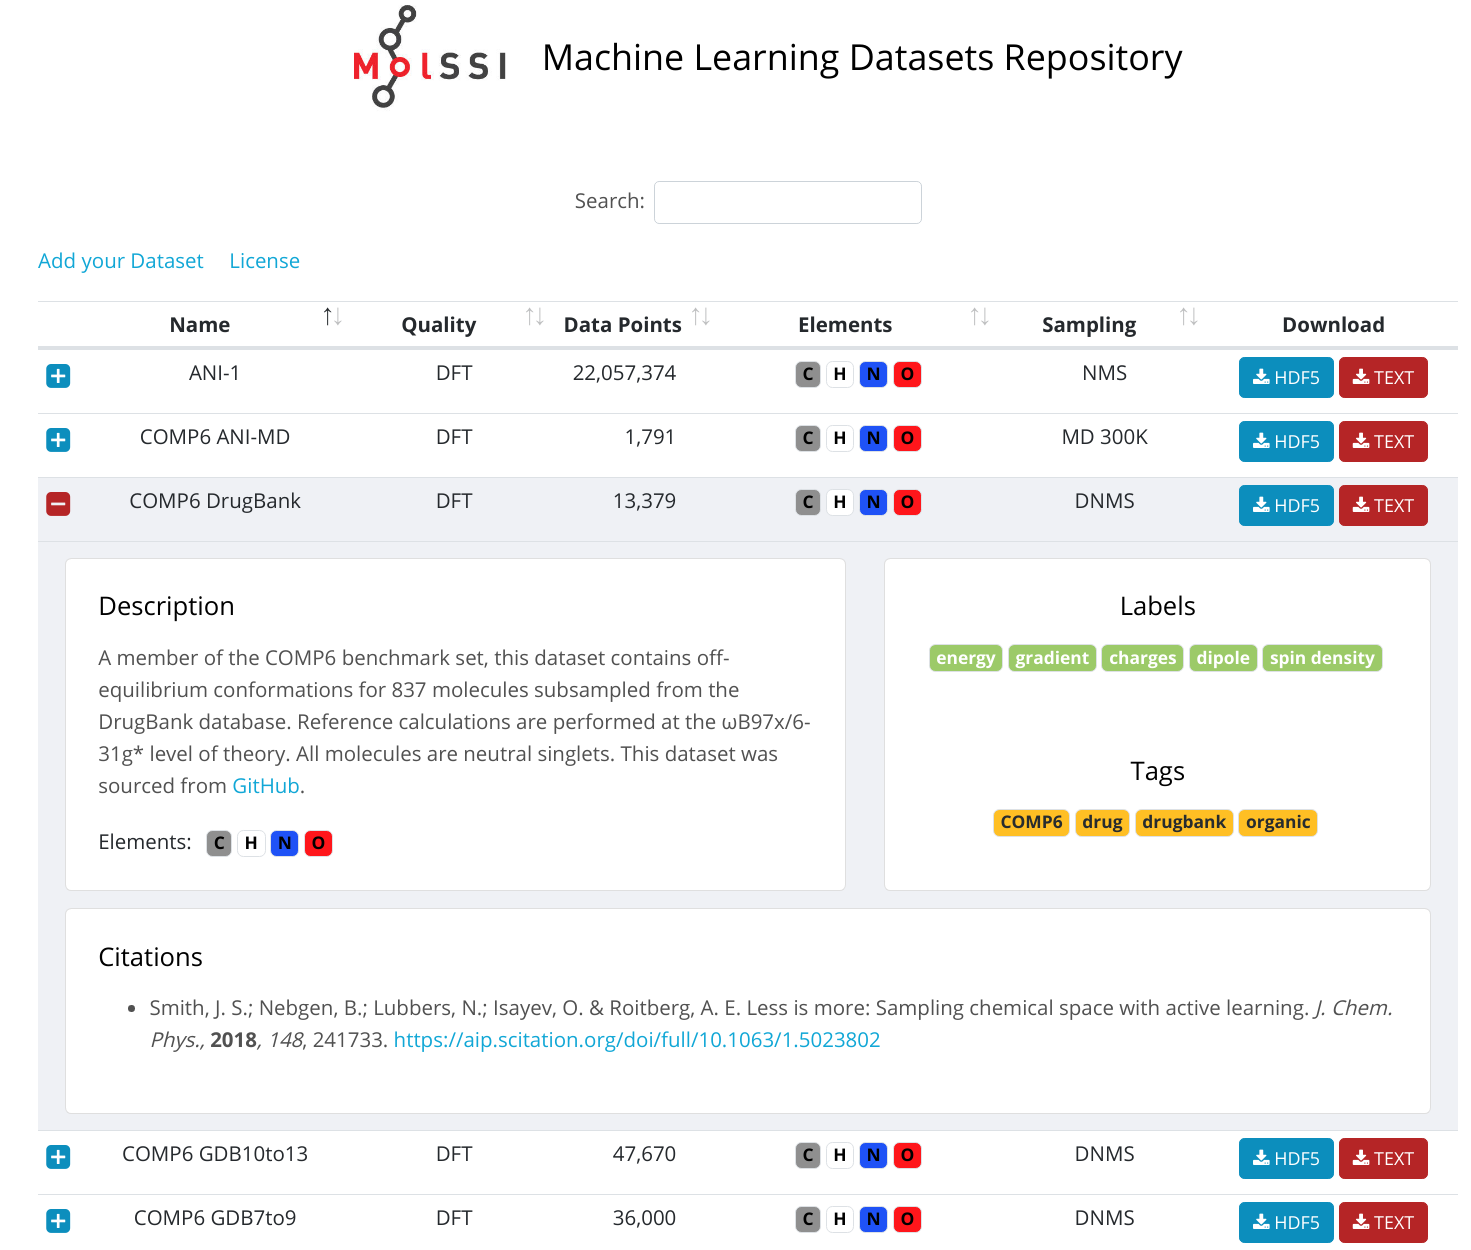
\includegraphics[width=0.9\textwidth]{./images/apps_ml_datasets.png}
\centering
\caption{QC Machine Learning Datasets Repository}
\label{fig:apps_ml_datasets}
\end{figure}


\subsection{Reaction Datasets Web App\label{sec:dbapp}}

The reaction datasets viewer app provides interactive visualization (see Fig.~\ref{fig:dbapp}) for benchmarking, providing statistics on hundreds of DFT and semiempirical methods for dozens of community benchmark datasets such as S22,\cite{Jurecka:2006:1985, Marshall:2011:194102}
HSG,\cite{Faver:2011:790, Marshall:2011:194102}
%PCONF,\cite{Reha:2005:6803, Smith:2016:2197}
ACONF,\cite{Gruzman:2009:11974}
HTBH,\cite{Zhao:2005:2012} and
SSI.\cite{Burns:2017:161727}

Analysis through the app can drive best practices for a given chemical problem while also considering user time and resource constraints. One can imagine pre-defined sets of tautomers, conformations, torsional scans, and dimers which have been pre-evaluated over several kinds and levels of theory, effectively providing a framework with which to quickly evaluate emerging methods

\begin{figure}[H]
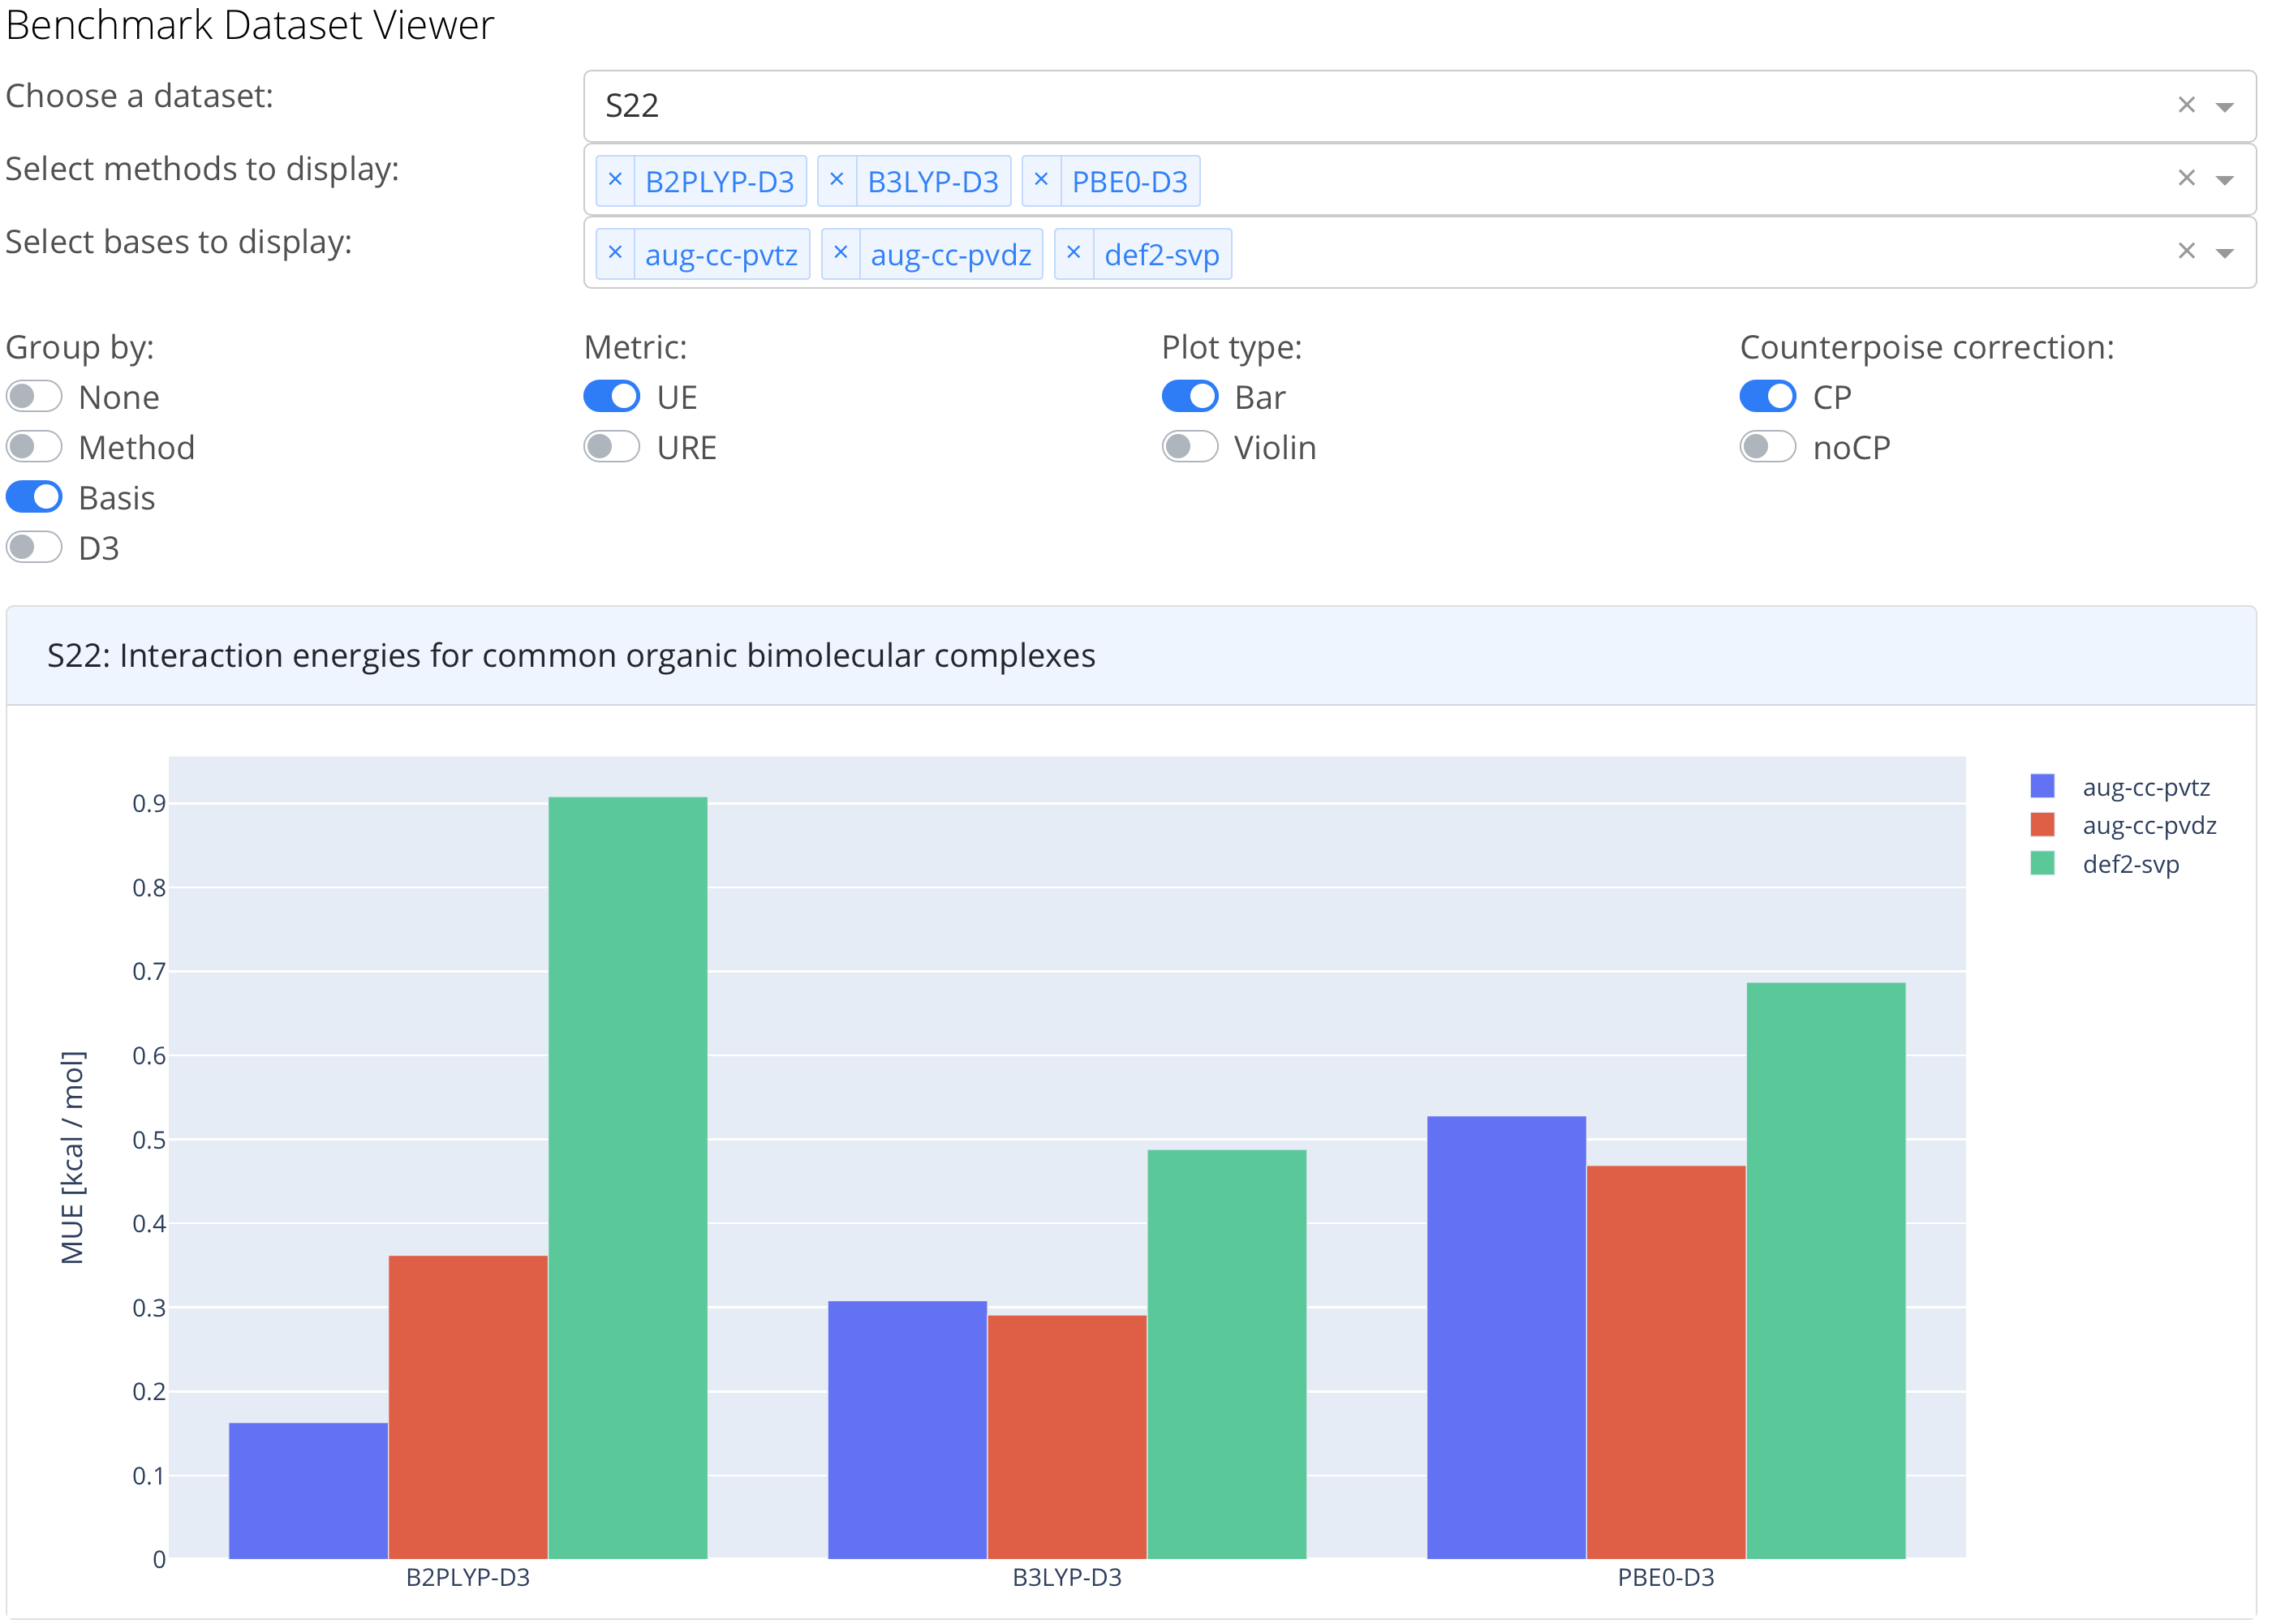
\includegraphics[width=0.9\textwidth]{./images/apps_reaction_datasets_v3.png}
\centering
\caption{Reaction Datasets Viewer app.
\label{fig:dbapp}}
\end{figure}

\subsection{Other Apps}

Additional apps are being developed based on their usefulness and input from the community.
For example, a common question that we have heard is the attempt to estimate the time a given quantum chemistry computation will take.
This is often hard for a human to accomplish as the steep scaling of quantum chemistry methods can easily mean the difference of one to two orders of magnitude.

The quantum chemistry execution time estimator app predicts the time of a quantum chemistry computation given a molecule (such as SMILES, InChI, or common file formats like XYZ), basis set, and level of theory.
In addition, time estimations will vary with respect to the number of threads provided and the physical hardware used.
The prediction is based on a machine learning model trained with hundreds of thousands of computations that exist in the \mqcas and is planned to be released shortly.

\section{Conclusions}

There is an urgent and growing need for data best-practices in the computational molecular sciences as the sheer number of quantum chemistry computations being evaluated across the community continues to grow exponentially.
This growth also puts a focus on the need for automation, replicability, and reproducibility\cite{NAP25303}.
The \qca addresses this need in the QC space through a MolSSI-hosted centralized data server (\mqcas) and a Python-based software infrastructure (\qcai).

The \mqcas represents an ongoing effort to gather, organize, host, and democratize quantum chemistry data for the benefit of the broader molecular sciences community. 
This goal is achieved first through FAIR data hosted by the \mqcas and through focusing on the areas of force-field fitting, methodological benchmarking, and machine learning.
These data are provided in full through either a Python or web interface.
To further broaden accessibility and utility of the \mqcas data, the QCArchive project is developing web apps that present chemical insights directly to users without the need for programming ability or data manipulation. 

The \qcai software is composed of a number of building blocks each at a different level of interaction from fully automated workflows on distributed computing to the conversion factor between units.
Independently, the software building blocks are in use by the community outside of the \qca (such as Psi4, geomeTRIC, and OpenFF) and the hope is these tools will power a larger software ecosystem built off of \qcsk.
When these building blocks are used together they create a unified platform for computing, structuring, and distributing computations and procedures at scale.

Taken together, these efforts have produced a substantial resource for the CMS community.
At the time of writing, the \mqcas contains 12 million molecules, 18 million calculation results (with full provenance information), and 96 data collections.
The \qcai demonstrates best practices in community-focused software development with 28 external code contributors, and use in 18 external software projects since its beta launch in August 2019.
We hope this kind of software infrastructure and data gathering methods will push CMS towards a more interoperable, data-driven, and computation commoditizing future.

\section{Acknowledgements}

We are grateful to Shantenu Jha, Matteo Turilli, Andre Merzky, Matt Horton, Lee-Ping Wang, Sebastian Lee, and John Chodera for helpful discussions.

\section{Funding Information}

D.G.A.S, D.A., M.W., L.N.N., S.E., and T.D.C.\ were supported by U. S. National Science Foundation (NSF) grant ACI-1547580.
L.A.B. was supported by NSF grant ACI-1449723.
L.W. developed capabilities for node-parallel applications and was supported by the Exascale Computing Project (17-SC-20-SC), a collaborative effort of the U.S. Department of Energy Office of Science and the National Nuclear Security Administration.
D.G.A.S. also acknowledges the Open Force Field Consortium and Initiative for financial and scientific support.

The contents of this paper are solely the
responsibility of the authors and do not necessarily represent the views of the NIH or the commercial partners of the Open Force Field Consortium.

\section{Research Resources}

The authors also acknowledge Advanced Research Computing at Virginia Tech, the Pacific Research Platform, the Open Science Grid, the Argonne Leadership Computing Facility, and the Memorial Sloan Kettering Institute for providing computational resources and technical support that have contributed to the results reported within the paper.

\bibliographystyle{unsrt} 
\bibliography{main}
\end{document}
